\chapter{Cosmic Rays}

\section{A Short History}

The discovery of cosmic rays has a long history.  The electroscope, a device
used to measure the amount of electrical charge in a body, has been crucial to
understanding the origin of this radiation.
As early as 1785, de Coulomb \cite{deCoulomb:1785} had found that an electroscope would
discharge spontaneously in the air due to some unknown action.  He
ruled out the effect of imperfect insulation.  This has been further studied by e.g.
\textcite{Faraday:1835} around 1835, and \textcite{Crookes:1879} in 1879.

A critical development was the discovery of X-rays in 1895 by
\textcite{Roentgen:1895}.  Röntgen performed experiments with different kinds of
cathode ray tubes.  At one point, he noted a faint glow from a nearby
fluorescent screen which he had prepared for one of his experiments.
Upon further investigation, he theorized the existence of invisible radiation
emanating from the tube, which he called X-rays.  Röntgen also discovered the
ionizing properties of X-rays, noting that air conducts electricity when
traversed by the radiation \cite{Flakus:1981}.

The component of X-ray tubes\footnote{Early designs for cathode ray tubes were later
optimized to efficiently produce X-rays.} responsible for the emission of X-rays
is also a source of fluorescence.
Becquerel extensively studied the possible connection between the emission of
visible light and X-rays.  For this, he used a uranium salt, known for its
strong phosphorescence.  This resulted in the discovery of spontaneous
radioactivity in 1896 \cite{Becquerel:1896}.  Becquerel found that, like X-rays, the new
radiation was also capable of ionizing dry air and discharging an electroscope.

Over the following years, many experiments were performed to study the emission
of ionizing radiation and its properties.  It remained a curious phenomenon that
a completely isolated electroscope would discharge slowly, even when no
X-ray tubes or radioactive materials were used in the currently-running experiment.
First observed by de Coulomb, it was now suspected that the environment itself
contained low levels of ionizing radiation.

In 1903 \textcite{RutherfordCooke:1903}, and independently
\textcite{McLennanBurton:1903}, enclosed their electroscopes in shields of metal
which they kept free from radioactive elements.  They found that the
electroscopes discharged more slowly.  Their conclusion was that the ionizing
radiation must come from outside the vessel and that it was not spontaneously generated
inside.

In 1909 \textcite{Kurz:1909} wrote a review on the origin of the ionizing
radiation.
He concluded that there were three options: a) the radiation was extra-terrestrial, b)
 it was an effect of radioactivity in the crust of the Earth, or c) it was an effect of radioactivity in the
atmosphere.  He concluded that the most likely option was the second one:
radioactive elements known to be present in the crust emit the ionizing
radiation measured by discharging electroscopes.
From this assumption, equations were derived describing the amount of ionizing
radiation as a function of height above the surface of the Earth.

Theodor Wulf, a German scientist and Jesuit priest teaching physics in the
Netherlands, designed an improved electroscope.  He visited Paris in 1909 and
measured the intensity of the radiation at the bottom and at the top
of the Eiffel Tower (\SI{300}{\meter}).  He found that the intensity of
the radiation decreased, but not nearly enough to confirm the
hypothesis of radiation coming from the Earth's crust \cite{Wulf:1909}.

Pacini questioned that same hypothesis. From 1907 to 1912 he measured the
intensity of radiation on both land and sea. If the radiation were coming from the
Earth's crust, a body of water above it should reduce the intensity by absorption.
Measurements at the surface of the sea did not show a reduction in the intensity of the radiation.  Pacini then
submerged an electroscope to a depth of \SI{3}{\meter} (the total depth of the
Gulf of Genoa at that location is \SI{8}{\meter}) \cite{Pacini:1912}.  He
measured a \SI{20}{\percent} decrease in discharge rate, consistent with the
hypotheses that the radiation was coming from above and was penetrating the
water. Pacini then derived the absorption rate for water from his measurements.

In 1909 \textcite{Gockel:1910} ascended in a balloon to \SI{4500}{\meter} and
found no decrease in the intensity of the radiation, at variance with the
then-accepted hypothesis that the radiation was coming from the surface of the
Earth.  In doing so, he confirmed Pacini's results.  However, many physicists were
reluctant to give up the established view.

Hess believed that resolving the dispute was of the highest importance.  First,
he carefully measured the absorption coefficient of gamma rays (believed
to be responsible for the penetrating radiation) through air \cite{Hess:1911}.
His results were in agreement with earlier measurements performed by
\textcite{Eve:1911}.  Now, having obtained an accurate absorption rate, he undertook a
series of balloon flights in 1911 and 1912, up to an altitude of
\SI{5200}{\meter} \cite{Hess:1912}.  His final results were that there was a
small decrease in the intensity of the radiation in the first few hundred meters above the
surface of the Earth.  Higher altitudes showed an increase in intensity. At
\SI{5200}{\meter}, the intensity of the radiation  was measured to be higher than at
ground level.  This was not at all consistent with the observed absorption
rates, under the assumption that the radiation was coming from the Earth's surface.  Hess concluded that the
radiation was of extra-terrestrial origin \cite{Hess:1913}.

\textcite{Kolhorster:1913} confirmed Hess' results in 1913--1914 by performing a
series of balloon flights with a maximum altitude of \SI{9200}{\meter}.  He also
calculated, in the assumption that the radiation was coming from above, the
absorption coefficient for air.  The result was eight times smaller than the
known absorption coefficient of \emph{gamma rays} for air.

\textcite{MillikanBowen:1923} developed small and light electroscopes which
could autonomously record a series of measurements on photographic film.
Instrumented, unmanned balloons took flights up to \SI{15000}{\meter} and found
intensities of only \num{1/4} of those measured by Hess and Kolhörster.  They
concluded in 1925 that at higher altitudes the intensity decreased again and
therefore, that the radiation was of terrestrial origin.  However, experiments
performed only one year later by \textcite{MillikanCameron:1926} using
electroscopes submerged in lakes at different altitudes, confirmed that the
radiation was coming from above.
It was Millikan who first proposed the term \emph{cosmic rays}.

Soon thereafter, Clay \cites{Clay:1927}{Clay:1928} found that ionization
increases with latitude, almost certainly caused by the magnetic field of the
Earth.  He concluded that gamma rays could not be the (only) source of cosmic
rays.  His results were disputed by Millikan.  When the Geiger-Müller counter
became available in 1928, the particle nature of cosmic rays was established by
\textcite{BotheKolhorster:1929}.
Millikan did not accept this interpretation.  When, in 1932,
\textcite{Compton:1933} performed a world-wide survey of cosmic ray intensities
and firmly established the dependence on latitude and the charged particle
nature of cosmic rays, Millikan attacked his views.  Finally, after performing
new experiments of his own, Millikan admitted in 1933 that cosmic rays indeed
(mostly) consisted of charged particles.

Cosmic rays have been instrumental in developing a coherent view of the particle
nature of our world.  Both antimatter (positrons) and the first examples of
other particle families (muons) were discovered in cosmic rays.  With the
discovery of \emph{extensive air showers} by \textcite{Auger:1939} in 1939 and
independently by Rossi \cite[5]{Rao:1998} in 1934 a new field of research was
established.

A recent review of the history of cosmic rays is given in \cite{Carlson:2011}.
The authors focus on the contributions of Pacini.


\section{Cosmic Rays in the Solar Neighborhood}
\label{sec:solar-neighborhood}

Cosmic particles continuously bombard the atmosphere of the Earth.  These
particles are called \emph{primary cosmic rays}, as they are not yet altered by
interactions in the atmosphere.

The composition and energy spectrum of primary cosmic rays have been studied
extensively.  For recent results, see e.g.
\cites{Takeda:2003}{Apel:2009}{Abraham:2010}{Bird:1993}. The most accurate
experiments make use of direct measurements, i.e. whereby the primary cosmic rays are
detected. To reduce the effect of the atmosphere, these experiments are usually
carried into the stratosphere using balloons, such as \cite{Boyle:2008}.  The
experiment is concluded when the balloon bursts.  The equipment falls back to
the surface, deploying a parachute to ensure a soft landing.  The experiment is
then recovered for analysis. It is also the case that experiments are being
conducted in space, such as \cite{George:2009}.

Charged cosmic rays consist mainly of protons (\SI{84}{\percent}) and alpha
particles (\SI{12}{\percent}). Most of the remainder are heavier nuclei.
Electrons make up less than \SI{1}{\percent} of cosmic rays
\parencite{Grupen:2005}.\footnote{Numbers are taken from \textcite[78,
84]{Grupen:2005}, but corrected here for \emph{total} composition, including
electrons.}  The chemical abundances are shown in
\figref{fig:composition}, along with the relative abundances of elements in the
Solar System.  Large similarities clearly exist.
\begin{figure}
\centering
{\pgfkeys{/artist/width/.initial=.95\linewidth}
% \usepackage{tikz}
% \usetikzlibrary{arrows}
% \usepackage{pgfplots}
% \pgfplotsset{compat=1.3}
% \usepackage[detect-family]{siunitx}
% \usepackage[eulergreek]{sansmath}
% \sisetup{text-sf=\sansmath}
% \usepackage{relsize}
%
\pgfkeysifdefined{/artist/width}
    {\pgfkeysgetvalue{/artist/width}{\defaultwidth}}
    {\def\defaultwidth{ \linewidth }}
%
%
\begin{sansmath}
\begin{tikzpicture}[
        font=\sffamily,
        every pin/.style={inner sep=2pt, font={\sffamily\smaller}},
        every label/.style={inner sep=2pt, font={\sffamily\smaller}},
        every pin edge/.style={<-, >=stealth', shorten <=2pt},
        pin distance=2.5ex,
    ]
    \begin{semilogyaxis}[
            width=\defaultwidth,
            axis equal=false,
            %
            title={  },
            %
            xlabel={ Nuclear Charge (Z) },
            ylabel={ Relative Abundance (Si = \num{e3}) },
            %
            xmin={  },
            xmax={  },
            ymin={  },
            ymax={  },
            %
            xtick={  },
            ytick={ 1e-6, 1e-4, 1e-2, 1e0, 1e2, 1e4, 1e6, 1e8 },
            %
            tick align=outside,
            max space between ticks=40,
            every tick/.style={},
            axis on top,
        ]

        

        

        
            
            % Draw series plot
            \addplot[mark=*,mark options=white,only marks] coordinates {
                (1.0, 29300000.0)
                (2.0, 2470000.0)
                (3.0, 0.0556)
                (4.0, 0.000612)
                (5.0, 0.0188)
                (6.0, 7190.0)
                (7.0, 2120.0)
                (8.0, 15700.0)
                (9.0, 0.804)
                (10.0, 3290.0)
                (11.0, 57.7)
                (12.0, 1030.0)
                (13.0, 84.6)
                (14.0, 1000.0)
                (15.0, 8.3)
                (16.0, 421.0)
                (17.0, 5.17)
                (18.0, 92.7)
                (19.0, 3.76)
                (20.0, 60.4)
                (21.0, 0.0344)
                (22.0, 2.47)
                (23.0, 0.286)
                (24.0, 13.1)
                (25.0, 9.22)
                (26.0, 848.0)
                (27.0, 2.35)
                (28.0, 49.0)
            };
        
            
            % Draw series plot
            \addplot[mark=o,solid] coordinates {
                (1.0, 29300000.0)
                (2.0, 2470000.0)
                (3.0, 0.0556)
                (4.0, 0.000612)
                (5.0, 0.0188)
                (6.0, 7190.0)
                (7.0, 2120.0)
                (8.0, 15700.0)
                (9.0, 0.804)
                (10.0, 3290.0)
                (11.0, 57.7)
                (12.0, 1030.0)
                (13.0, 84.6)
                (14.0, 1000.0)
                (15.0, 8.3)
                (16.0, 421.0)
                (17.0, 5.17)
                (18.0, 92.7)
                (19.0, 3.76)
                (20.0, 60.4)
                (21.0, 0.0344)
                (22.0, 2.47)
                (23.0, 0.286)
                (24.0, 13.1)
                (25.0, 9.22)
                (26.0, 848.0)
                (27.0, 2.35)
                (28.0, 49.0)
            };
        
            
            % Draw series plot
            \addplot[mark=*,solid] coordinates {
                (1.0, 977654.0)
                (2.0, 193669.0)
                (3.0, 1027.2)
                (4.0, 498.9)
                (5.0, 1803.8)
                (6.0, 7337.0)
                (7.0, 1713.7)
                (8.0, 7082.6)
                (9.0, 101.8)
                (10.0, 998.7)
                (11.0, 189.6)
                (12.0, 1368.2)
                (13.0, 202.7)
                (14.0, 1000.0)
                (15.0, 26.2)
                (16.0, 157.0)
                (17.0, 24.9)
                (18.0, 58.8)
                (19.0, 41.6)
                (20.0, 124.8)
                (21.0, 26.0)
                (22.0, 100.4)
                (23.0, 45.7)
                (24.0, 98.8)
                (25.0, 61.4)
                (26.0, 653.7)
                (27.0, 3.7)
                (28.0, 27.8)
            };
        

        

        

        
            \node[coordinate,
                  pin={[pin distance=3.5ex] above:{ O }}]
                at (axis cs:8, 15700.0) {};
        
            \node[coordinate,
                  pin={[pin distance=3.5ex] above:{ Si }}]
                at (axis cs:14, 1000.0) {};
        
            \node[coordinate,
                  pin={[pin distance=3.5ex] above:{ Fe }}]
                at (axis cs:26, 848.0) {};
        
            \node[coordinate,
                  pin={[pin distance=3.5ex] above:{ Li }}]
                at (axis cs:3, 1027.2) {};
        
            \node[coordinate,
                  pin={[pin distance=3.5ex] above:{ Be }}]
                at (axis cs:4, 498.9) {};
        
            \node[coordinate,
                  pin={[pin distance=3.5ex] above:{ B }}]
                at (axis cs:5, 1803.8) {};
        
            \node[coordinate,
                  pin={[pin distance=3.5ex] above:{ C }}]
                at (axis cs:6, 7337.0) {};
        
            \node[coordinate,
                  pin={[pin distance=3.5ex] above:{ Sc }}]
                at (axis cs:21, 26.0) {};
        
            \node[coordinate,
                  pin={[pin distance=3.5ex] above:{ Ti }}]
                at (axis cs:22, 100.4) {};
        
            \node[coordinate,
                  pin={[pin distance=3.5ex] above:{ V }}]
                at (axis cs:23, 45.7) {};
        
            \node[coordinate,
                  pin={[pin distance=4.5ex] above:{ Cr }}]
                at (axis cs:24, 98.8) {};
        
            \node[coordinate,
                  pin={[pin distance=3.5ex] above:{ Mn }}]
                at (axis cs:25, 61.4) {};
        

        

    \end{semilogyaxis}
\end{tikzpicture}
\end{sansmath}
}
\caption{\captitle{Relative abundances of elements in the Solar System and in
cosmic rays.}  The relative abundances are normalized, with the abundance of Si
set to \num{1000}.  Two datasets are shown: relative abundances
of elements in the Solar System (open circles), and relative abundances of
galactic cosmic rays (GCR) measured by the CRIS instrument on the NASA/ACE
satellite ($Z \geq 3$) and the BESS balloon experiment ($Z \leq 2$),
during a solar minimum (closed circles).  The plot is redrawn from
\cite{George:2009}, using data from
\cites{George:2009}{Lodders:2009}{Wang:2002}{deNolfo:2006}.}
\label{fig:composition}
\end{figure}
However, the light elements Li, Be and B are much more abundant, as well as the
sub-iron elements Sc, Ti, V, Cr and Mn.  This is attributed to
\emph{spallation}, the splitting of nuclei due to interactions in the
interstellar medium (ISM).  The most abundant elements in the universe are H,
He, C, O and Fe.  Spallation of C and O will thus increase the abundances of Li,
Be and B.  Similarly, the sub-iron elements are produced in spallation of Fe.

Another feature which is evident in both the solar system abundances and the
cosmic ray abundances is the difference between elements with even and odd
atomic numbers.  An explanation for this can be found by considering the
\emph{shell model} of the nucleus.  Nuclear configurations with an even number
of protons and neutrons (considered separately) are more stable than
odd-numbered configurations.  If the total number of nucleons is a so-called
\emph{magic number}, i.e.
\numlist[list-final-separator={ or }]{2;8;20;28;50;82;126}, then the nucleus is
extremely stable.

Antiparticles are extremely rare in cosmic rays
\parencites{Smoot:1975}{Picozza:2003}. This is further corroboration for the
observation that the universe seems to consist only of matter, without any
regions made up of antimatter.  The antimatter that \emph{is} found in
cosmic rays is produced by the interaction of cosmic rays with the ISM.  For
example, antinucleons can be produced by proton-proton collisions.
Positrons are produced by pair creation, i.e.
\begin{equation}
\HepProcess{\Pphoton^* \,\to\, \Pelectron + \Ppositron}.
\end{equation}
Only one in every \num{10000} charged nucleons is an antiproton
\parencite{Picozza:2003}. Positrons are relatively more abundant, for every
ten electrons there is one positron.

The particle flux strongly depends on the energy of the particle.  Low-energy
particles are deflected by the magnetic fields of the Earth and the Sun. Very
low-energy particles get trapped in the Van Allen radiation belts surrounding
the Earth.  These particles leak away when they enter the atmosphere near the
magnetic poles.  Interactions between these particles and air molecules produce the
spectacular aurorae.  These particles stem mainly from the solar wind, the stream
of particles ejected from the upper atmosphere of the Sun. Solar wind particles
are predominantly protons and electrons in the \si{\mega\electronvolt} energy
range \parencite{Grupen:2005} and where the solar wind encounters the magnetic field of
the Earth,
the interaction region is called the \emph{magnetosphere}. The properties of the
magnetosphere strongly depend on solar activity and thus follow the solar cycle
\parencite{Nagashima:1989}, which lasts eleven years.
Furthermore, the solar wind, as it is a \emph{plasma}, carries the magnetic
field of the Sun into the entire solar system and beyond, throughout the
\emph{heliosphere}.  Therefore, the so-called \emph{interplanetary magnetic
field} also strongly depends on the solar cycle.
The particle fluxes of low-energy primary cosmic rays thus follow this same
cycle.  When solar activity is high, fewer cosmic rays reach the Earth.  For
particle energies larger than \SI{10}{\giga\electronvolt}, solar modulation is
no longer apparent.

The energy spectrum of primary cosmic rays is shown in
\figref{fig:energy_spectrum}.
\begin{figure}
\centering
{\pgfkeys{/artist/width/.initial=.6\linewidth}
\pgfkeys{/artist/height/.initial=.8\linewidth}
% \usepackage{tikz}
% \usetikzlibrary{arrows}
% \usepackage{pgfplots}
% \pgfplotsset{compat=1.3}
% \usepackage[detect-family]{siunitx}
% \usepackage[eulergreek]{sansmath}
% \sisetup{text-sf=\sansmath}
% \usepackage{relsize}
%
\pgfkeysifdefined{/artist/width}
    {\pgfkeysgetvalue{/artist/width}{\defaultwidth}}
    {\def\defaultwidth{ .5\linewidth }}
%
\pgfkeysifdefined{/artist/height}
    {\pgfkeysgetvalue{/artist/height}{\defaultheight}}
    {\def\defaultheight{ .65\linewidth }}
%
\begin{sansmath}
\begin{tikzpicture}[
        font=\sffamily,
        every pin/.style={inner sep=2pt, font={\sffamily\smaller}},
        every label/.style={inner sep=2pt, font={\sffamily\smaller}},
        every pin edge/.style={<-, >=stealth', shorten <=2pt},
        pin distance=2.5ex,
    ]
    \begin{axis}[
            xmode=log,
            ymode=log,
            width=\defaultwidth,
            height=\defaultheight,
            axis equal=false,
            %
            title={  },
            %
            xlabel={ Energy [\si{\electronvolt}] },
            ylabel={ Flux [\si{\per\square\meter\per\steradian\per\second\per\giga\electronvolt}] },
            %
            xmin={  },
            xmax={  },
            ymin={  },
            ymax={  },
            %
            xtick={ 1e6, 1e9, 1e12, 1e15, 1e18, 1e21 },
            ytick={  },
            %
            tick align=outside,
            max space between ticks=40,
            every tick/.style={},
            axis on top,
        ]

        




    
    % Draw series plot
    \addplot[no markers,solid] coordinates {
        (212000000.0, 3920.0)
        (299000000.0, 4440.0)
        (422000000.0, 4240.0)
        (597000000.0, 3680.0)
        (843000000.0, 2820.0)
        (1190000000.0, 1954.0)
        (1680000000.0, 1264.0)
        (2380000000.0, 750.0)
        (3360000000.0, 414.0)
        (4220000000.0, 266.0)
        (5320000000.0, 162.4)
        (7300000000.0, 80.8)
        (9940000000.0, 38.6)
        (12900000000.0, 19.92)
        (18200000000.0, 8.2)
        (22700000000.0, 4.58)
        (25900000000.0, 3.24)
        (30000000000.0, 2.18)
        (35800000000.0, 1.372)
        (44100000000.0, 0.788)
        (57400000000.0, 0.392)
        (82400000000.0, 0.1538)
    };

    
    % Draw series plot
    \addplot[no markers,solid] coordinates {
        (316200000000.0, 0.00576887304264)
        (993900000000.0, 0.0002550600612)
        (3.839e+12, 5.44528998815e-06)
        (1.84e+13, 8.60394451508e-08)
        (3.724e+13, 1.60555423349e-08)
        (5.218e+13, 5.55840374252e-09)
        (9.451e+13, 1.22895992304e-09)
        (1.847e+14, 2.27711459446e-10)
        (3.164e+14, 5.24065641597e-11)
        (6.146e+14, 1.10861432718e-11)
        (1.074e+15, 2.21815879083e-12)
    };

    
    % Draw series plot
    \addplot[no markers,solid] coordinates {
        (4.786e+14, 1.96834282935e-11)
        (5.495e+14, 1.21920756201e-11)
        (6.761e+14, 7.96080917976e-12)
        (8.318e+14, 3.44284934316e-12)
        (1.023e+15, 2.28200352072e-12)
        (1.259e+15, 1.15852176479e-12)
        (1.549e+15, 7.07724940383e-13)
        (1.905e+15, 3.96539372777e-13)
        (2.344e+15, 2.39957157774e-13)
        (2.884e+15, 1.52056638942e-13)
        (3.548e+15, 8.77082404407e-14)
        (4.365e+15, 5.58389220544e-14)
        (5.37e+15, 3.19257536328e-14)
        (6.457e+15, 1.64777537967e-14)
        (7.943e+15, 8.20472208718e-15)
        (9.772e+15, 4.51889258037e-15)
        (1.202e+16, 2.54252989189e-15)
        (1.479e+16, 1.12998149387e-15)
        (1.82e+16, 7.34136945226e-16)
        (2.239e+16, 3.24256734098e-16)
        (2.754e+16, 1.9102627533e-16)
        (3.388e+16, 1.06937943363e-16)
        (4.169e+16, 5.44383960065e-17)
        (5.129e+16, 3.01246953922e-17)
        (6.31e+16, 1.67866485509e-17)
        (7.762e+16, 8.95575203332e-18)
        (9.55e+16, 4.46730719587e-18)
        (1.175e+17, 2.42020636757e-18)
        (1.202e+17, 2.2091142592e-18)
        (1.445e+17, 1.34996415989e-18)
        (1.514e+17, 1.11073038421e-18)
        (1.778e+17, 7.64241485916e-19)
        (1.905e+17, 5.52466278264e-19)
        (2.188e+17, 3.34861433819e-19)
        (2.399e+17, 2.68526605145e-19)
        (2.692e+17, 1.76950733309e-19)
        (3.02e+17, 1.35207056767e-19)
        (3.311e+17, 1.14053637664e-19)
        (3.802e+17, 6.87026324113e-20)
        (4.074e+17, 4.98795925018e-20)
        (4.786e+17, 3.06267524287e-20)
        (6.026e+17, 1.71341513353e-20)
        (7.586e+17, 7.96051879073e-21)
        (9.55e+17, 3.42711291851e-21)
        (1.202e+18, 1.70367445308e-21)
        (1.514e+18, 9.24217919144e-22)
    };

    
    % Draw series plot
    \addplot[no markers,solid] coordinates {
        (4.742e+17, 3.16083509028e-20)
        (1.37e+18, 1.35274789393e-21)
        (3.467e+18, 6.79513033958e-23)
        (7.824e+18, 7.06663967142e-24)
        (1.593e+19, 1.11523974549e-24)
        (2.585e+19, 3.36358091822e-25)
        (3.744e+19, 8.90963072531e-26)
    };

    
    % Draw series plot
    \addplot[no markers,solid] coordinates {
        (1.647e+17, 1.23613875451e-18)
        (2.276e+17, 4.67759516871e-19)
        (3.44e+17, 1.28635437246e-19)
        (5.026e+17, 4.29160975591e-20)
        (7.141e+17, 1.51463412486e-20)
        (9.663e+17, 5.51831831788e-21)
        (1.29e+18, 2.1373374041e-21)
        (1.979e+18, 6.87396651365e-22)
        (2.968e+18, 1.73726920055e-22)
        (3.929e+18, 5.58498765336e-23)
        (5.245e+18, 2.21199725949e-23)
        (7.766e+18, 6.73103276605e-24)
        (1.052e+19, 3.02311318854e-24)
        (1.615e+19, 1.06295576346e-24)
        (2.048e+19, 8.53045609146e-25)
        (3.154e+19, 1.68433274478e-25)
        (4.6e+19, 4.24738371572e-26)
        (6.38e+19, 9.35125842718e-27)
        (8.773e+19, 1.38634426817e-26)
        (1.177e+20, 1.15238895403e-26)
    };

    
    % Draw series plot
    \addplot[no markers,solid] coordinates {
        (1.995e+17, 4.19845874947e-19)
        (2.512e+17, 1.98160255495e-19)
        (3.162e+17, 1.02117378909e-19)
        (3.981e+17, 5.17617965457e-20)
        (5.012e+17, 2.3328664545e-20)
        (6.31e+17, 1.07116641622e-20)
        (7.943e+17, 5.22597167309e-21)
        (1e+18, 2.63007524745e-21)
        (1.259e+18, 1.14495928428e-21)
        (1.585e+18, 5.87282593098e-22)
        (1.995e+18, 2.53605561582e-22)
        (2.512e+18, 1.21321890028e-22)
        (3.162e+18, 5.23702580781e-23)
        (3.981e+18, 3.25110418571e-23)
        (5.012e+18, 1.33034815931e-23)
        (6.31e+18, 8.14546156628e-24)
        (7.943e+18, 4.3553116493e-24)
        (1e+19, 2.23351671138e-24)
        (1.259e+19, 1.31496080924e-24)
        (1.585e+19, 8.91085787697e-25)
        (1.995e+19, 4.36687213039e-25)
        (2.512e+19, 1.09881368828e-25)
        (3.162e+19, 5.74219617308e-26)
        (3.981e+19, 4.77533084336e-26)
        (3.162e+20, 6.34021270919e-28)
    };

    
    % Draw series plot
    \addplot[no markers,dashed] coordinates {
        (100000000000.0, 0.0843511987786)
        (132571136559.0, 0.0388469176707)
        (175751062485.0, 0.0178904749947)
        (232995181052.0, 0.00823924045267)
        (308884359648.0, 0.00379448188252)
        (409491506238.0, 0.00174750243539)
        (542867543932.0, 0.000804790971793)
        (719685673001.0, 0.000370636684198)
        (954095476350.0, 0.000170692212621)
        (1.26485521686e+12, 7.86102204445e-05)
        (1.67683293681e+12, 3.62029799921e-05)
        (2.22299648253e+12, 1.66728416851e-05)
        (2.94705170255e+12, 7.67847425595e-06)
        (3.90693993705e+12, 3.53622783763e-06)
        (5.17947467923e+12, 1.6285666791e-06)
        (6.86648845004e+12, 7.5001655721e-07)
        (9.10298177992e+12, 3.45410994408e-07)
        (1.20679264064e+13, 1.59074828297e-07)
        (1.59985871961e+13, 7.32599755287e-08)
        (2.12095088792e+13, 3.37389898322e-08)
        (2.81176869797e+13, 1.55380810147e-08)
        (3.72759372031e+13, 7.15587404422e-09)
        (4.94171336132e+13, 3.29555067246e-09)
        (6.5512855686e+13, 1.51772574079e-09)
        (8.68511373751e+13, 6.98970112495e-10)
        (1.15139539933e+14, 3.21902175755e-10)
        (1.52641796718e+14, 1.48248128073e-10)
        (2.02358964773e+14, 6.82738705492e-11)
        (2.68269579528e+14, 3.14426998868e-11)
        (3.55648030622e+14, 1.44805526363e-11)
        (4.71486636346e+14, 6.66884222435e-12)
        (6.25055192527e+14, 3.07125409715e-12)
        (8.28642772855e+14, 1.41442868371e-12)
        (1.09854114199e+15, 6.51397910439e-13)
        (1.4563484775e+15, 2.99993377262e-13)
        (1.93069772888e+15, 1.38158297653e-13)
        (2.5595479227e+15, 6.36271219875e-14)
        (3.3932217719e+15, 2.93026964082e-14)
        (4.49843266897e+15, 1.34950000875e-14)
        (5.96362331659e+15, 6.21495799653e-15)
        (7.90604321091e+15, 2.86222324181e-15)
        (1.04811313415e+16, 1.31816206811e-15)
        (1.38949549437e+16, 6.07063492614e-16)
        (1.84206996933e+16, 2.79575700879e-16)
        (2.44205309455e+16, 1.28755185368e-16)
        (3.23745754282e+16, 5.9296633102e-17)
        (4.29193426013e+16, 2.73083424731e-17)
        (5.68986602902e+16, 1.25765246628e-17)
        (7.54312006335e+16, 5.7919653216e-18)
        (1e+17, 2.66741911506e-18)
    };







    \node[coordinate,,
          pin={ above right:{ LEAP }}]
        at (axis cs:4179569355.81, 272.957831791) {};

    \node[coordinate,,
          pin={ above right:{ PROTON }}]
        at (axis cs:1.84282066409e+13, 8.59346675067e-08) {};

    \node[coordinate,,
          pin={ above right:{ AGASA }}]
        at (axis cs:2.69184026272e+16, 2.07106994388e-16) {};

    \node[coordinate,,
          pin={ below left:{ Yakutsk }}]
        at (axis cs:5.24224614953e+18, 4.31440358167e-23) {};

    \node[coordinate,,
          pin={ below left:{ Haverah Park }}]
        at (axis cs:4.39201721077e+19, 6.05909845321e-26) {};

    \node[coordinate,,
          pin={ below left:{ Fly's Eye }}]
        at (axis cs:3.162e+20, 6.34021270919e-28) {};




    \end{axis}
\end{tikzpicture}
\end{sansmath}
}
\caption{\captitle{Differential flux of primary cosmic rays as a function
of particle energy.}  The dashed line corresponds to a spectral index
$\gamma$ = $2.75$.  The figure shows the results from several
experiments, indicated by the labels.  LEAP is a balloon-borne
experiment; PROTON is a satellite and the other experiments are
ground-based arrays.  The data from several experiments overlap.  Figure
redrawn from \textcite{Cronin:1997}.}
\label{fig:energy_spectrum}
\end{figure}
Except for the low-energy region ($E < \SI{10}{\giga\electronvolt}$), the
spectrum follows a power law, i.e. $F(E) \sim E^{-\gamma}$, with the
spectral index $\gamma \sim 3$.  It is assumed that this feature of the spectrum
largely originates at the source, i.e. it is the result of the acceleration process.

Cosmic rays are predominantly produced inside our Galaxy and are contained by
the galactic magnetic field.  Above a certain energy threshold, cosmic rays
start to leak away and the spectrum becomes steeper.  This is a probable
explanation for the so-called \emph{knee} in the cosmic ray spectrum. At the
knee ($E \approx \SI{4}{\peta\electronvolt}$), the spectral index $\gamma$
changes from \num{2.7} to \num{3.1} \cite{Amenomori:2008}.
Another explanation is that at the knee, the maximum energy at which cosmic ray
particles can be accelerated by the sources in the galaxy is reached.
Both explanations may play an important role.  See \textcite{Hoerandel:2004} for
a detailed overview of models explaining the knee.  Since both magnetic
confinement and maximum attainable energy are proportional to charge, heavier
nuclei in the galaxy must be observed to have larger maximum energies than
protons.  It means that while protons start to leak away, heavier nuclei like
iron are still bound to the galaxy.  In a particular source, heavy nuclei can be
accelerated to higher energies than protons.  Therefore, at energies around the
knee, the composition of the spectrum changes slowly from proton to iron \parencite{Bird:1993}.
At energies significantly above the knee, cosmic rays must originate from
extra-galactic sources.

At even higher energies, the spectrum becomes less steep.  This region is
called the \emph{ankle}.  At these energies, the flux is so low that
measurements of the spectrum show very low statistics.

Greisen, Zatsepin and Kuzmin predicted that ultra-high energy cosmic rays
(UHECRs) will interact with the cosmic microwave background (CMB).  At
ultra-high energies, the available energy in a collision between a cosmic ray
particle and a CMB photon is above the so-called \emph{pion production
threshold}:
\begin{align}
\HepProcess{\Pproton + \Pphoton_{CMB} &\to \PgD^+ \to \Pproton +
\Ppizero}, \\
\HepProcess{\Pproton + \Pphoton_{CMB} &\to \PgD^+ \to \Pneutron +
\Ppiplus}.
\end{align}
Each collision results in a loss of energy for the cosmic ray particle. The
process continues until the available energy becomes lower than the pion
production threshold.  For UHECR protons, the GZK limit is
\SI{50}{\exa\electronvolt}. The mean free path for a proton with an energy of
\SI{60}{\exa\electronvolt} is \SI{10}{\mega\parsec}.  If there are protons above
this energy, they cannot have traveled farther than about \SI{50}{\mega\parsec},
since their energy would have been reduced by the GZK effect.  Similar arguments
hold for heavier nuclei and photons. The latter lose energy due to pair
production:
\begin{equation}
\HepProcess{\Pphoton + \Pphoton_{CMB} \to \Pelectron + \Ppositron}.
\end{equation}
The GZK effect should result in a pile-up of cosmic rays with an energy below
the GZK limit, similar to the pile-up of sub-iron nuclei which is observed in
the \emph{composition} of cosmic rays. This pile-up is most likely responsible
for the smaller slope of the spectrum around the ankle.

If cosmic ray sources above the GZK limit exist that are closer than
\SI{50}{\mega\parsec}, a proportion of them should be detected.
Thus, if the limit is observed, it proves that at these energies, the
majority of cosmic ray sources are indeed more than \SI{50}{\mega\parsec} away.
Cosmic ray particles, produced with energies above the GZK limit and
originating at those sources, drop below the limit before they
reach the Earth.

To put these numbers into perspective, the diameter of the Milky Way is
approximately \SI{35}{\kilo\parsec} and the largest distance within the
\emph{local supercluster}\footnote{The Local Supercluster contains the Virgo
cluster and the Local Group.  The latter comprises more than 50 galaxies,
including the Andromeda galaxy and the Milky Way.  The Local Supercluster
contains more than 100 galaxy groups and clusters.} is only
\SI{30}{\mega\parsec}.


\section{Production}


\subsection{Sources}

The galactic magnetic field deflects cosmic ray particles.  At energies below
\SI{100}{\tera\electronvolt}, the direction of arrival is not correlated to the
direction of the source.  At these energies, the distribution of cosmic rays
becomes highly isotropic.  To try and find a source of cosmic ray particles
at a distance of \SI{10}{\mega\parsec}, the evolution of
the galactic magnetic field over the last 50 million years would need to be known.
At energies above \SI{e19}{\electronvolt}, however, the direction of arrival
should be in correlation with the direction of the source.  No correlation with the
galactic plane is found, however, which is further proof for extra-galactic sources.
Recently, the Auger collaboration reported \cite{Abreu:2010} on their current
results regarding the correlation of UHECRs with
active galactic nuclei (AGNs).  Events with estimated energies above
\SI{55}{\exa\electronvolt} are reconstructed and their origins are compared to
the positions of known AGNs within \SI{75}{\mega\parsec}, as recorded in the
12$^{\mathrm{th}}$ edition of the Véron-Cetty and Véron catalog
\cite{VCV-catalog}.  If the origin of an event is closer than \SI{3.1}{\degree}
to the position of an AGN, it is counted as a \emph{correlation}.  The Auger
collaboration reports 21 correlations out of 55 events
(\SI{38}{\percent}) \cite{Abreu:2010}.  The correlation fraction is down from an
early estimate of \SI{69}{\percent}, which was derived from 9 correlations out
of 13 events.
The correlation fraction which is expected from an isotropic distribution of events
is \SI{21}{\percent}.  The collaboration emphasizes that further research should
be done.

If the direction of arrival can be used to pinpoint sources, it should be noted
that the small deflections caused by intergalactic magnetic fields in combination with
the large distances traveled results in significant time lags when compared to
the arrival time of neutral particles like photons and neutrinos.  For example, when
$\gamma$-ray bursts (GRB) produce charged cosmic rays, they arrive months or
even years later than the photons and neutrinos produced in the same event
\cite[85]{Grupen:2005}.

In order to identify the sources of cosmic rays, \textcite{Hillas:1984} studied
the various possible acceleration mechanisms and noted that they all need strong
magnetic fields and large sizes.  In the case of direct acceleration, rotating
magnetic fields provide electric fields which accelerate charged particles.  The
stronger the field and the larger its size, the more energy a particle can
acquire.  For statistical acceleration models, in which acceleration occurs in
many small steps, the amount of energy that a particle gains depends on the
ability of the accelerator to \emph{contain} the particles.  Statistical
acceleration can occur at a shock wave front, resulting from e.g. supernovas.
If particles are contained by magnetic fields, they can cross the front many
times and slowly gain energy.

Charged particles contained in a uniform magnetic field rotate with a radius
\begin{equation}
r = \frac{m\beta c}{ZB},
\end{equation}
called the \emph{Larmor radius}, with $m, Z$ the particle mass and atomic number
(or charge), $\beta c$ the particle velocity perpendicular to the magnetic
field, and $B$ the strength of the magnetic field.  For particles to acquire
large energies, the source should have strong magnetic fields or a large size.
In particular, the source should be larger than the Larmor radius.
If the source is very large, magnetic fields of the order of \si{\micro\gauss}
are sufficient to accelerate particles.

Hillas found \cite{Hillas:1984} that for statistical acceleration models the
approximate upper limit on the energy is given by
\begin{equation}
E_{15} \leq 0.5 \beta_s Z B_{\si{\micro\gauss}} L_{\si{\parsec}},
\end{equation}
with $E_{15}$ the energy in units of \SI{e15}{\electronvolt},
$B_{\si{\micro\gauss}}$ the magnetic field of the source in \si{\micro\gauss},
$\beta_s$ the velocity of the shock wave relative to $c$ and
$L_{\si{\parsec}}$ the size of the source in \si{\parsec}.  When the
magnetic field of the sources is plotted versus the size of the sources,
one obtains the \emph{Hillas plot} shown in \figref{fig:Hillas}.
\begin{figure}
\centering
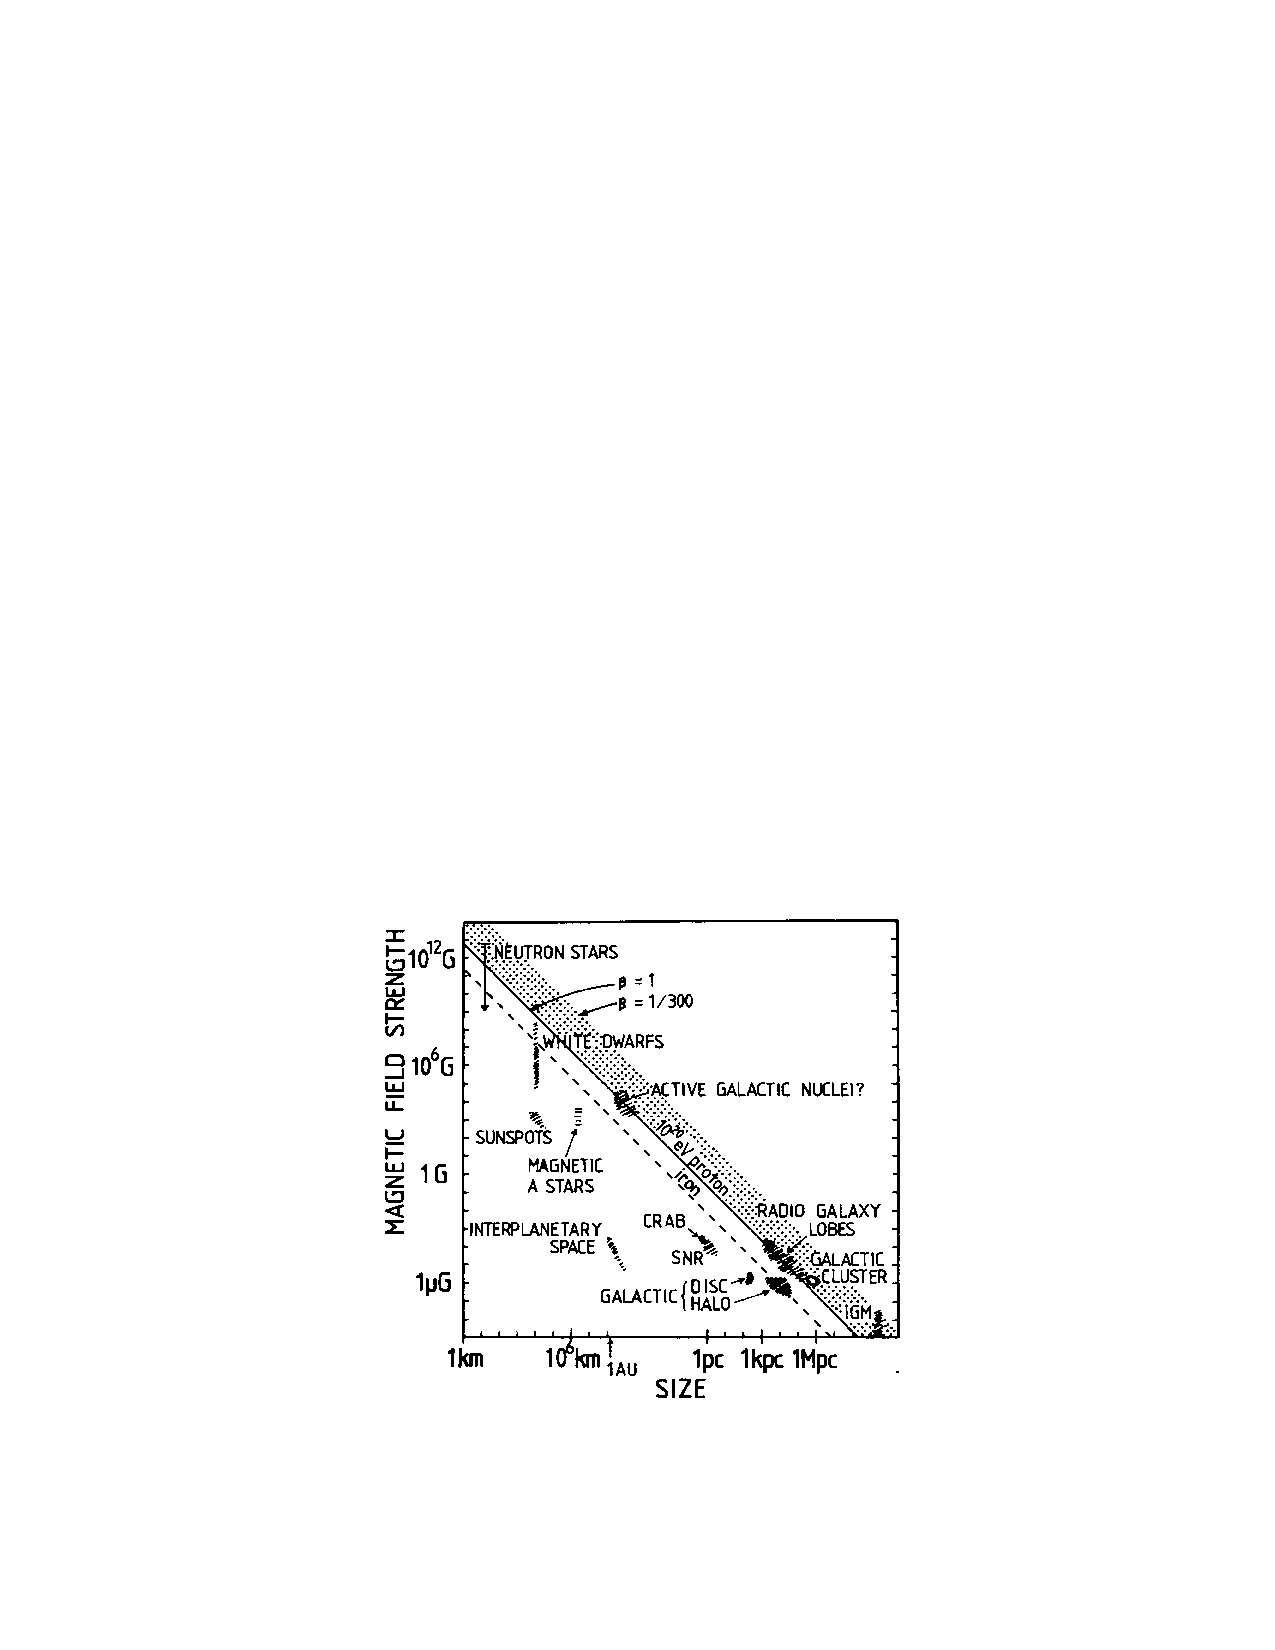
\includegraphics[width=.7\linewidth]{raw-plots/Hillas-plot}
\caption{\captitle{Hillas plot.}  The size and magnetic field strength of
possible acceleration sites are shown in the plot.  The diagonal line shows the limit
for \SI{e20}{\electronvolt} protons, i.e. sources below that line can not
accelerate protons to this limit.  The dashed line shows the limit for
\SI{e20}{\electronvolt} iron nuclei.  Reproduced from \cite{Hillas:1984}.}
\label{fig:Hillas}
\end{figure}
It is obvious that not many sources accelerate charged particles to the
highest energies.

Alternative models that do not require a large size and a strong
magnetic field are so-called \emph{top-down models}, as opposed to the
bottom-up acceleration models discussed thus far.  Top-down models suggest that
ultra-high energy cosmic rays are produced by the decay of highly energetic
exotic objects \cite{Olinto:2000}.  These should be relics of the
Big Bang and none of them have been observed.

Candidate sources should not only accelerate particles to the highest
energies, the totality of sources should also reproduce the observed power law
spectrum.
Finally, sources should be able to fill the galaxy with enough cosmic rays to
produce an energy density of \SI{1}{\electronvolt\per\meter\cubed}
\cite[11]{Gaisser:1990}.


\subsection{Acceleration Mechanisms}

Currently, acceleration is favored above decay models.  This leaves open
the question of \emph{how} cosmic rays are accelerated to ultra-high energies.
Such a mechanism must not only be realistic, but should also reproduce the
cosmic ray energy spectrum.  There are many possible acceleration sites, including sun
spots and pulsars with high magnetic fields.
In particular, pulsars are able to accelerate particles due to
their rotating magnetic fields, which generate strong electric fields.
Particles are accelerated along so-called \emph{jets}.

Other processes work more slowly, but over long time scales.  These provide an
energy spectrum similar to the observed spectrum of cosmic rays up to the knee.

Two acceleration models will be discussed in the following sections. In
each section, simple considerations will lead to the development of a
basic model. Similar calculations can be found in the literature
\cite[67--68]{Grupen:2005}. Those calculations, however, contain errors (a
missing factor of two in parts of the equations), which have been repeated
by others.


\subsubsection{Fermi Acceleration}

Two well-known candidate models are Fermi acceleration and shock acceleration.  Fermi
supposed \cite{Fermi:1949} that the interstellar medium is filled with turbulent
magnetic fields, with high fields being found mainly in interstellar clouds.
These fields can act as a \emph{magnetic mirror}.  In such a configuration,
charged particles encounter varying field strengths when moving along magnetic
field lines.  This results in the particles being deflected away from regions
with strong fields.  In Fermi's model, charged particles encounter magnetic
clouds and eventually leave the cloud, being scattered in the process.  If the
particle exits the cloud traveling in its original direction, its energy remains
unchanged as all scattering in a magnetic field is \emph{elastic}.  However,
if the direction of the particle is \emph{changed}, this does not need to be the
case.
All magnetic interactions are elastic only in the reference frame of the
cloud.\footnote{In the cloud frame the velocity of the cloud is zero, and it
contains only magnetic fields. In the lab frame, however, a non-zero cloud
velocity will result in electric fields. Hence, the collisions will no longer
be elastic.} To determine the energy in the lab frame, two
transformations must be performed: one from the lab frame to the cloud frame and
one from the cloud frame back to the lab frame.

As a simple model calculation, consider a particle with velocity $v$
traveling towards a magnetic cloud which itself is approaching with velocity
$-u$.  The situation is depicted in the top part of
\figref{fig:fermi-2nd-order}.
\begin{figure}
\centering
\begin{tikzpicture}
[font=\sffamily,
]
\draw[very thick,gray] (0, -5) -- (0, 2);


\node at (0, 0) [left=20pt] (lab) {\begin{tikzpicture}
\node[anchor=center] at (1.5, 2) {Lab frame};

\draw[fill] (0, -10pt) circle (1pt);
\draw[->] (0, -10pt) -- +(2, 0) node[midway,below] {$v$};
\draw[gray] (2cm+2pt, -10pt) -- (3cm-8pt, -10pt) to[out=0,in=0,looseness=3] (3cm-8pt, 10pt);
\node[draw, cloud, minimum width=55pt, minimum height=45pt, anchor=center] at (3, 0) {};
\draw[->] (3, 0) -- +(-.75, 0) node[midway,below] {$-u$};

\draw[fill] (3cm-10pt, 10pt) circle (1pt);
\draw[->,dashed] (3cm-10pt, 10pt) -- +(-3.5, 0) node [midway,above] {$-(v + u) - u$};
\end{tikzpicture}};

\node at (0, 0) [right=20pt] (cloud) {\begin{tikzpicture}
\node[anchor=center] at (1.5, 2) {Cloud frame};

\draw[fill] (0, -10pt) circle (1pt);
\draw[->] (0, -10pt) -- +(2.75, 0) node[midway,below] {$v + u$};
\draw[gray] (2.75cm+2pt, -10pt) to[out=0,in=0,looseness=3] (2.75cm+2pt, 10pt) -- (3cm-8pt, 10pt);

\draw[fill] (3cm-10pt, 10pt) circle (1pt);
\draw[->,dashed] (3cm-10pt, 10pt) -- +(-2.75, 0) node[midway,above] {$-(v + u)$};
\node[draw, cloud, minimum width=55pt, minimum height=45pt, anchor=center] at (3, 0) {};
\end{tikzpicture}};

\node at (0, 0) [below left=70pt and 20pt] {\begin{tikzpicture}

\draw[fill] (0, -10pt) circle (1pt);
\draw[->] (0, -10pt) -- +(2, 0) node[midway,below] {$v$};
\draw[gray] (2cm+2pt, -10pt) -- (3cm-8pt, -10pt) to[out=0,in=0,looseness=3] (3cm-8pt, 10pt) -- (2cm-18pt, 10pt);
\node[draw, cloud, minimum width=55pt, minimum height=45pt, anchor=center] at (3, 0) {};
\draw[->] (3, 0) -- +(.75, 0) node[midway,below] {$u$};

\draw[fill] (2cm-20pt, 10pt) circle (1pt);
\draw[->,dashed] (2cm-20pt, 10pt) -- +(-.5, 0) node [midway,above] {$-(v - u) + u$};
\end{tikzpicture}};

\draw[very thick,gray] (0, -2) -- (0, 2);

\node at (0, 0) [below right=70pt and 20pt] {\begin{tikzpicture}

\draw[fill] (0, -10pt) circle (1pt);
\draw[->] (0, -10pt) -- +(1.25, 0) node[midway,below] {$v - u$};
\draw[gray] (1.25cm+2pt, -10pt) -- (3cm-8pt, -10pt) to[out=0,in=0,looseness=3] (3cm-8pt, 10pt) -- (2cm-18pt, 10pt);

\draw[fill] (2cm-20pt, 10pt) circle (1pt);
\draw[->,dashed] (2cm-20pt, 10pt) -- +(-1.25, 0) node[midway,above] {$-(v - u)$};
\node[draw, cloud, minimum width=55pt, minimum height=45pt, anchor=center] at (3, 0) {};
\end{tikzpicture}};

\end{tikzpicture}
\caption{\captitle{Fermi acceleration mechanism.}  In the top part of the
figure, a particle with velocity $v$ moves towards a magnetic cloud with
velocity $-u$.  In the frame of the magnetic cloud, the velocity remains
unchanged when the particle is reflected back.  However, in the lab frame
the particle has gained velocity, and thus kinetic energy.  In the bottom
part of the figure, the cloud moves with a velocity $u$ and is overtaken
by the particle.  In that case, the particles \emph{loses} energy.}
\label{fig:fermi-2nd-order}
\end{figure}
The kinetic energy of the particle is then given by $E_0 = \frac{1}{2} m
v^2$.  In the frame of the magnetic cloud, the particle's
velocity is given by $v + u$.  When reversed, this becomes $-(v + u)$.  Finally,
in the original lab frame, the particles velocity has become $-(v + u) - u = -v
- 2u$.  With this, the particle's kinetic energy is now given by
\begin{equation}
E_1 = \frac{1}{2} m (-v - 2u)^2 = \frac{1}{2} m (v^2 + 4u^2 + 4uv)
\end{equation}
while the energy gain becomes
\begin{equation}
\Delta E_1 = E_1 - E_0 = \frac{1}{2} m (4u^2 + 4uv).
\end{equation}
%
However, it is also possible that the particle encounters a cloud moving in the
same direction with velocity $u$, i.e. a \emph{rear-end collision}.  That
situation is shown in the bottom part of \figref{fig:fermi-2nd-order}.  In
this case, the particle's velocity in the cloud
frame becomes $v - u$ and reversed, $-(v - u)$.  In the lab frame, this becomes
 $-(v - u) + u = -v + 2u$.  The kinetic energy is then given by
\begin{equation}
E_2 = \frac{1}{2} m (-v + 2u)^2 = \frac{1}{2} m (v^2 + 4u^2 - 4uv),
\end{equation}
and the energy gain by
\begin{equation}
\Delta E_2 = E_2 - E_0 = \frac{1}{2} m (4u^2 - 4uv).
\end{equation}
If the particle's velocity is higher than the
cloud's velocity, i.e. $v > u$, the energy `gain' $\Delta E_2$ is negative and
the particle has \emph{lost} energy.  If $v < u$, it is
impossible for the particle to overtake a magnetic cloud.

Under the assumption that the velocity $v$ is much greater than $u$, the
particle will experience approximately the same number of head-on collisions and
rear-end collisions.  The mean energy gain over the two
types of collisions is given by:
\begin{equation}
\frac{\Delta E_1 + \Delta E_2}{E_0} = \frac{\frac{1}{2} m (8u^2)}{\frac{1}{2} m
v^2} = 8\frac{u^2}{v^2}
\end{equation}
which is proportional to the square of the velocity of the magnetic cloud.
Therefore, this model of acceleration is also referred as \emph{second order
Fermi acceleration}.

If there are many clouds with randomized velocities and directions and the
particles velocity $v$ is still smaller than the mean cloud velocity $u$, the
probability of a head-on encounter is higher than that of a rear-end
encounter. This means that the probability of an energy gain is higher than
that of an energy loss.

There is a probability that the particle escapes
from the magnetic cloud region.  Taking the energy gain per collision and the
probability of a further collision, one can calculate the resulting energy
spectrum, which happens to be a power law \cite[75]{Grupen:2005}.  The spectral
index depends on the magnetic cloud velocities and the probability of the
particle escaping the region of acceleration \cite{Grupen:2005}.  Fermi
acceleration requires long time scales, and therefore may not work in practice.


\subsubsection{Shock Acceleration}

During supernova explosions, stellar matter is ejected at very high speeds into
the interstellar medium.  This heats up the interstellar matter, increasing
its density and pressure and driving the matter outward.  The emerging
\emph{shock wave} travels faster than the supernova ejecta following it.
Both stellar and interstellar matter are \emph{plasmas} and it is the
electromagnetic fields that cause the shock wave, not collisions in the plasma.
In fact, the particle densities are so low that the matter is called
\emph{collisionless}.

As seen from the perspective of the shock front (\figref{fig:fermi-1st-order}),
upstream (\emph{unshocked}) gas flows towards the front at a velocity of
$u_1$ and a density of $\rho_1$.  Since the density $\rho_2$ of the downstream
(\emph{shocked}) gas is higher, it is possible to calculate its velocity
$u_2$.
\begin{figure}
\centering
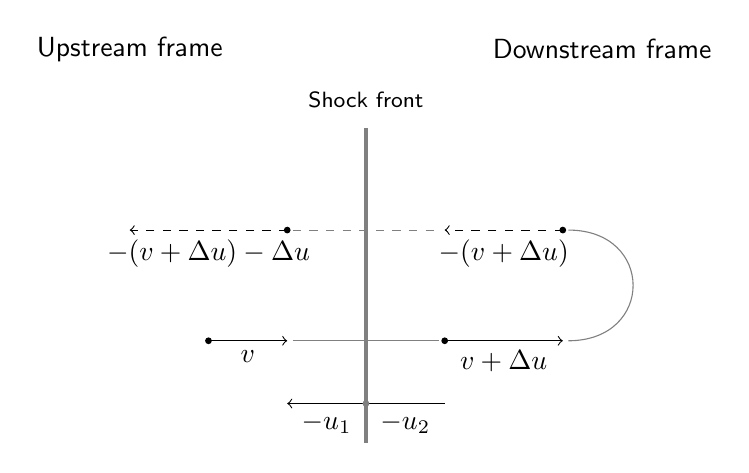
\begin{tikzpicture}
[font=\sffamily,
]

\draw[very thick,gray] (0, -2) -- (0, 2);
\node at (-3, 3) {Upstream frame};
\node at (3, 3) {Downstream frame};
\node at (0, 2cm+10pt) {\footnotesize Shock front};

\draw[->] (1, -1.5) -- +(-2, 0) node[near end,below] {$-u_1$} node[near start,below] {$-u_2$};;
\draw[fill,gray] (0, -1.5) circle (1pt);

\begin{scope}[yshift=-20pt]
\draw[gray] (-1cm+2pt, 0) -- (1cm-2pt, 0);
\draw[fill] (-2, 0) circle (1pt);
\draw[->] (-2, 0) -- +(1, 0) node[midway,below] {$v$};
\draw[fill] (1, 0) circle (1pt);
\draw[->] (1, 0) -- +(1.5, 0) node[midway,below] {$v + \Delta u$};
\end{scope}

\begin{scope}[yshift=20pt]
\draw[gray,dashed] (-1cm+2pt, 0) -- (1cm-2pt, 0);
\draw[fill] (2.5, 0) circle (1pt);
\draw[->,dashed] (2.5, 0) -- +(-1.5, 0) node[midway,below] {$-(v + \Delta u)$};
\draw[fill] (-1, 0) circle (1pt);
\draw[->,dashed] (-1, 0) -- +(-2, 0) node[midway,below] {$-(v + \Delta u) - \Delta u$};
\end{scope}

\draw[gray] (2.5cm+2pt, -20pt) to[out=0,in=0,looseness=2] (2.5cm+2pt, 20pt);

\end{tikzpicture}

\caption{\captitle{Shock acceleration mechanism.}  A shock front is moving
through the interstellar medium with velocity $-u_1$ in the upstream frame, and
$-u_2$ in the downstream frame.  A particle with velocity $v$ in the upstream
frame crosses the front.  Downstream, it is reflected and in that frame
the velocity remains unchanged.  However, in the original upstream frame, it
has gained velocity, and thus energy.}
\label{fig:fermi-1st-order}
\end{figure}
As the shock front is immaterial, any matter flowing into the front must also
exit the front. Therefore,
\begin{equation}
\rho_1 u_1 = \rho_2 u_2,
\end{equation}
and since $\rho_2 > \rho_1$, then $u_2 < u_1$.  Let $\Delta u =
u_1 - u_2$, which is a positive number.  The frame of the upstream gas is shown
in the left part of \figref{fig:fermi-1st-order}, with the frame of the
downstream gas shown in the right part.

The situation is now very similar to the situation described by second order Fermi
acceleration.  A particle can cross the shock front and be deflected by
magnetic fields inside the shocked gas.  If its velocity is larger than the
velocity of the shock front, it may cross the shock front again, resulting in
\begin{equation}
E_1 = \frac{1}{2} m (-v - 2\Delta u)^2 = \frac{1}{2} m (v^2 + 4\Delta u^2 +
4v\Delta u),
\end{equation}
giving the energy gain
\begin{equation}
\Delta E_1 = E_1 - E_0 = \frac{1}{2} m (4\Delta u^2 + 4v\Delta u).
\end{equation}
%
The difference between Shock and Fermi acceleration is that the probability of encountering
a \emph{receding} shock wave is, in this situation, zero.  Unlike magnetic
clouds, the shock wave travels in only one direction: outward.  The relative
energy gain is thus given by
\begin{equation}
\frac{\Delta E_1}{E_0} = \frac{\frac{1}{2} m (4\Delta u^2 +
4v\Delta u)}{\frac{1}{2} m v^2} = 4\left(\frac{\Delta u^2}{v^2} +
\frac{\Delta u}{v}\right).
\end{equation}
Given the velocity $v \gg \Delta u$, the linear term dominates:
\begin{equation}
\frac{\Delta E_1}{E_0} \sim \frac{4\Delta u}{v}.
\end{equation}
Because of the magnetic fields present in the plasma on both sides of the shock front,
and the fact that the particle's velocity is higher than the velocity of the
shock, the particle can cross the shock front countless times.  Shock
acceleration is sometimes called \emph{Fermi acceleration of the first order} and
is believed to be the primary process for cosmic ray production.


\section{Propagation}

Cosmic rays propagate from their source through the interstellar medium (ISM).
The ISM consists of matter, magnetic fields and radiation fields.  Charged
particles interact with the magnetic fields. Matter interacts with matter and
produces secondary particles. Additionally, electrons emit synchrotron
radiation caused by magnetic acceleration and lose energy through
Brehmsstrahlung and inverse Compton scattering.

The interstellar matter mainly consists of hydrogen, the most common form of which is
atomic hydrogen (\hi).  This can be observed by the \SI{21}{\centi\meter}
spectral line, resulting from the hyperfine splitting of hydrogen energies.
In dense regions, such as \emph{giant molecular clouds}, the outer parts of a cloud
absorb the energetic interstellar photons.  As a result, the inner parts are
shielded and in such regions molecules can be formed without breaking up.
Since cold H$_2$ is hard to detect, carbon monoxide (CO) is usually used as a
tracer for H$_2$ \cite{Combes:1997}. In clouds with an embedded infrared source,
one can observe both H$_2$ and CO absorption lines, and the H$_2$ / CO ratio can
be obtained \parencite{Lacy:1994}. This ratio is then assumed to be
approximately correct for all molecular clouds.  For a study of the relationship
between H$_2$ and CO, see e.g. \textcite{Glover:2011}.
In these dense regions, star formation can occur. Newly formed stars break up
the cloud with their radiation and stellar winds and in these regions, hydrogen is
ionized (denoted as \hii).

In the galactic arms, atomic hydrogen has an average density of
\SI{1}{atom\per\centi\meter\cubed} and a scale height\footnote{Distance over
which the density decreases by a factor of $e$.  Note that the \emph{thickness}
is twice the height.} of \SIrange{100}{150}{\parsec}.  Between the arms, the
density decreases by a factor of \numrange{2}{3}.  Molecular hydrogen is
concentrated within the solar circle\footnote{The solar circle is the orbit of
the Sun around the galactic center.} and especially in the region of the galactic
center.  In giant molecular clouds, the average density is of the order of
\SIrange[allow-number-unit-breaks]{1e2}{1e5}{atom\per\centi\meter\cubed}.
Ionized hydrogen only makes up a small fraction of the interstellar matter. The
average interstellar matter density is \SI{1}{nucleon\per\centi\meter\cubed}
\cite[75]{Stanev:2004}.

The large-scale structure and strength of the magnetic fields in the galaxy are
unknown.  Most knowledge is gathered by studying other galaxies; in particular
galaxies which are perpendicular to our line of sight.  By observing the Faraday
rotation of linearly polarized signals from radio pulsars, which is caused by
the magnetic field, the galactic distribution of the fields can be studied.  It
is believed that the magnetic field of the Milky Way is similar to that of other
galaxies.  Fluctuations in the field strength are, however, quite large. The
magnetic field near the Solar System is about \SI{1.8}{\micro\gauss}
for the regular component, which is uniform over a large region of space
\cite{Han:2000}.  The total field strength, which includes random fields on
smaller scales, is about \SI{5}{\micro\gauss}.

Ionized gas and magnetic fields carried by the gas form a
\emph{magnetohydrodynamic (MHD) fluid}.  This fluid can support \emph{Alfvén
waves}.  These waves can be created by cosmic rays streaming into the ISM.
Alfvén waves can scatter cosmic rays and under certain conditions
\emph{self-confinement} can occur: cosmic rays stream into the ISM, create
Alfvén waves which then scatter and even contain the particles to the
acceleration region.  The creation of such waves may even be essential to
cosmic ray acceleration through shocks.

The abundance of the unstable nucleus $^{10}$Be, which is created by spallation
of heavy cosmic ray nuclei, can be used to calculate the confinement time of
(heavy) cosmic rays in the galaxy. It is of the order of \SI{e7}{\year}
\cite[85]{Stanev:2004}.


\section{Cosmic Rays in the Atmosphere}
\label{sec:showers}

On average, primary cosmic rays in the ISM traverse a column
density of only a few \si{\gram\per\centi\meter\squared}.  In contrast, the
atmosphere of the Earth has a column density of
\SI{1030}{\gram\per\centi\meter\squared}.

When discussing cosmic rays in the atmosphere, it is common to refer to the
\emph{atmospheric depth} $X$, instead of the height $h$ above sea level.  The
atmospheric depth is the amount of matter above the atmospheric layer at height
$h$. Like column density, the atmospheric depth is measured in
\si{\gram\per\centi\meter\squared} and is defined by
\begin{equation}
X \equiv \int_h^\infty \rho(h') \,\ud h'.
\end{equation}

For a perfect gas with a constant temperature in hydrostatic equilibrium, the
profile is given by \cite[122]{Stanev:2004}
\begin{equation}
X = X_0 \exp\left(\frac{-h}{h_0}\right),
\end{equation}
where $X_0$ the atmospheric depth at sea level
(\SI{1030}{\gram\per\centi\meter\cubed}) and $h_0$ the scale height of the
atmosphere.

The temperature of the atmosphere is not constant.  The US Standard Atmosphere
\cite{atmosphere:1976} is a collection of models defining temperature, pressure,
density and several other observable qualities of the atmosphere over a wide range of
altitudes. Using these models, the altitude-dependent atmospheric density can be
approximated by dividing the atmosphere in several layers. Within each layer a
linear fit of the temperature to the experimentally observed values is made.
Then, the other properties of the atmosphere can be calculated.

When cosmic rays enter the atmosphere with a zenith angle $\theta$, the amount
of atmosphere traversed is called the \emph{slant depth} and is, in the
\emph{flat Earth approximation}, given by
\begin{equation}
X' = X / \cos\theta,
\end{equation}
with $X$ sometimes referred to as the \emph{vertical depth}.
This approximation is valid for zenith angles less than \SI{60}{\degree}. For
larger angles, the curvature of the Earth must be taken into account.

The radiation length\footnote{The mean distance over which the energy of a
high-energy electron is reduced to a factor $1/e$. This is approximately $7/9$
of the mean free path of pair-production for a high-energy photon.} in air is
\SI{36.66}{\gram\per\centi\meter\squared} and the interaction
length\footnote{The mean distance before a high-energy hadron
undergoes a hadronic interaction.} in air is
\SI{90.0}{\gram\per\centi\meter\squared}.
The total atmospheric depth is therefore approximately 28 radiation lengths and
11 interaction lengths.  The first interaction of primary cosmic rays with the
atmosphere is at a height of about \SIrange{15}{20}{\kilo\meter}.


\subsection{Interactions}

Cosmic rays traversing the atmosphere (or any substance of matter) can undergo
many different types of interactions.

Photons, for example, lose energy through \emph{Compton scattering} (photons
interacting with electrons, ionizing the atoms) and \emph{pair production}
(photons creating a particle-anti-particle pair in the vicinity of a nucleus).

Charged particles lose energy through \emph{ionization losses} (charged
particles transferring energy to atomic electrons thus exciting or ionizing the
atoms), \emph{Bremsstrahlung} (charged particles radiating photons while
interacting with the electromagnetic field of atomic nuclei), and
\emph{Rutherford scattering} (deflection by Coulomb forces).  Smaller losses are
due to \emph{synchrotron radiation} (charged particles deflected by the
Earth's magnetic field radiate photons), and the \emph{Cherenkov effect}
(charged particles traveling faster than the \emph{phase velocity} of light in a
medium emit radiation in a cone).

For hadrons, the situation is more complicated because of the many possible types of
interactions. Hadronic processes include nuclear fragmentation, creation of
resonances, and multiparticle production.
Furthermore, these processes are harder to calculate.  At very high energies,
QCD perturbation theory can be used to calculate cross sections.  At lower
energies, perturbation theory breaks down and effective theories must be used
\cite{Pythia:1987}. However, at these energies experimental data is available
from (collider) experiments. Approximations are made by measuring many cross
sections at different energies and the resulting models describe the data very
well.

When primary cosmic rays interact with the atmosphere they produce secondary
particles.  These particles will also interact and produce tertiary particles.
This process continues and the total number of particles increases dramatically
until the individual particle energies drop below the energy at which new
particles can be created.  Low-energy particles are absorbed in the
atmosphere.  The totality of particles created in this process is called a
\emph{cascade}.  If a large number of secondary particles reaches ground
level, the cascade is called an \emph{extensive air shower (EAS)} which
can have a footprint of several \si{\kilo\meter\squared}.


\subsection{Electromagnetic Cascades}

Cascades are called \emph{electromagnetic} when they consist of electrons and
photons.  They are initiated either by cosmic ray electrons and photons, or by
electrons and photons created as secondary particles in hadronic interactions
from cosmic ray nuclei.

At high energies, Bremsstrahlung
\begin{equation}
\HepProcess{\Pe \to \Pe + \Pphoton}
\end{equation}
and pair production
\begin{equation}
\HepProcess{\Pphoton^* \to \Pelectron + \Ppositron}
\end{equation}
dominate.

This process is surprisingly well described by the Heitler model.  This
model describes a cascade consisting of a single type of particle interacting
exactly after an interaction length $\lambda$.  Each interaction creates two
particles with equal energy, which is half the parent energy.  Thus, a
primary particle with energy $E_0$ will interact after one length $\lambda$ to
create two particles, each with energy $E = E_0 / 2$.  After two interaction
lengths, there are four particles with energy $E = E_0 / 2^2$; after three
interaction lengths, there are eight particles with energy $E = E_0 / 2^3$, and so
on.

The Heitler model \cite{Heitler:1954} describes an electromagnetic cascade
qualitatively until the particle energy drops below the critical energy at which
no more particles can be created.  It does not describe the absorptive
processes.  Ionization losses mean that electrons and positrons lose energy
rapidly until they annihilate (positrons with atomic electrons) or recombine
(electrons with ionized atoms).
Photons will be absorbed in Compton scattering and the photoelectric effect. A
generalization of the Heitler model is discussed in \cite{Montanus:2011}, which
does describe absorptive processes and can be used to describe the full
longitudinal development of an electromagnetic shower.


\subsection{Hadronic Cascades}

Hadronic cascades are created by cosmic ray protons and nuclei interacting with
the atmosphere.  Hadronic interactions and decays mainly result in the creation
of pions and kaons, for example
\begin{equation}
\HepProcess{\Pproton + \Pproton \to \Pproton + \PgD^+ \to \Pproton + \Pproton +
\Ppizero},
\end{equation}
where the $\PgD^+$ resonance can also decay into a neutron and a charged pion.
The pion to kaon production ratio is approximately 9:1.  Pions mainly decay to
muons, electrons, neutrinos, and photons, e.g.
\begin{equation}
\begin{split}
\HepProcess{\Ppiplus &\to \APmuon + \Pnum}, \\
\HepProcess{\Ppiminus &\to \Pmuon + \APnum}, \\
\HepProcess{\Ppizero &\to \Pphoton + \Pphoton}.
\end{split}
\end{equation}
Kaons have many decay modes \cite{Cirigliano:2012} and mainly decay to pions,
muons, electrons and neutrino's. At relativistic energies, the decay of pions and
kaons is retarded, in the lab frame, due to \emph{time dilation}. At
these energies, interactions with matter can occur before the particles decay.
However, at lower energies, decay is the dominant process.

The photons produced by decaying neutral pions initiate electromagnetic
cascades.  Furthermore, electromagnetic cascades can be created by electrons and
positrons resulting from decaying muons
\begin{equation}
\begin{split}
\HepProcess{\Pmuon &\to \Pelectron + \APnue}, \\
\HepProcess{\APmuon &\to \Ppositron + \Pnue}.
\end{split}
\end{equation}

The largest fraction of the primary energy ultimately goes towards the production
of electromagnetic cascades.


\subsection{Longitudinal and Lateral Shower Profiles}

To obtain an accurate description of the evolution of a shower,
\textcite{Rossi:1941} solved a set of diffusion equations describing the
development of electromagnetic cascades for various approximations.
Qualitatively, the longitudinal development can be parametrized by
\cite[157]{Grupen:2005}
\begin{equation}
N(t) \sim t^\alpha \exp(-\beta t),
\end{equation}
with $N(t)$ being the number of particles at $t = x / X_0$ the shower depth in
radiation lengths, and $\alpha$ and $\beta$ being free fit parameters parameterizing
the creation and absorption of particles respectively.
\figref{fig:longitudinal_distribution} shows the longitudinal development of an
EAS initiated by a \SI{1}{\peta\electronvolt} proton.
\begin{figure}
\centering
% \usepackage{tikz}
% \usetikzlibrary{arrows}
% \usepackage{pgfplots}
% \pgfplotsset{compat=1.3}
% \usepackage[detect-family]{siunitx}
% \usepackage[eulergreek]{sansmath}
% \sisetup{text-sf=\sansmath}
% \usepackage{relsize}
%
\pgfkeysifdefined{/artist/width}
    {\pgfkeysgetvalue{/artist/width}{\defaultwidth}}
    {\def\defaultwidth{ .5\linewidth }}
%
%
\begin{sansmath}
\begin{tikzpicture}[
        font=\sffamily,
        every pin/.style={inner sep=2pt, font={\sffamily\smaller}},
        every label/.style={inner sep=2pt, font={\sffamily\smaller}},
        every pin edge/.style={<-, >=stealth', shorten <=2pt},
        pin distance=2.5ex,
    ]
    \begin{axis}[
            xmode=normal,
            ymode=log,
            width=\defaultwidth,
            axis equal=false,
            %
            title={  },
            %
            xlabel={ Atmospheric depth [\si{\gram\per\centi\meter\squared}] },
            ylabel={ Number of particles },
            %
            xmin={  },
            xmax={  },
            ymin={  },
            ymax={  },
            %
            xtick={  },
            ytick={  },
            %
            tick align=outside,
            max space between ticks=40,
            every tick/.style={},
            axis on top,
        ]

        




    
    % Draw series plot
    \addplot[no markers,smooth] coordinates {
        (51.8062, 9251.61)
        (103.611, 99545.5)
        (155.416, 500195.0)
        (207.221, 1419235.0)
        (259.026, 2796906.0)
        (310.831, 4280570.0)
        (362.636, 5438811.0)
        (414.441, 6086355.0)
        (466.246, 6196028.0)
        (518.051, 5946996.0)
        (569.856, 5418979.0)
        (621.661, 4811922.0)
        (673.465, 4148159.0)
        (725.27, 3506044.0)
        (777.075, 2921480.0)
        (828.88, 2405365.0)
        (880.685, 1960832.0)
        (932.49, 1573544.0)
        (984.295, 1238545.0)
    };

    
    % Draw series plot
    \addplot[no markers,smooth] coordinates {
        (51.8062, 841.588)
        (103.611, 10758.4)
        (155.416, 51631.1)
        (207.221, 139188.0)
        (259.026, 261561.0)
        (310.831, 383117.0)
        (362.636, 470382.0)
        (414.441, 511453.0)
        (466.246, 515179.0)
        (518.051, 485411.0)
        (569.856, 439551.0)
        (621.661, 385842.0)
        (673.465, 330769.0)
        (725.27, 277578.0)
        (777.075, 230140.0)
        (828.88, 188636.0)
        (880.685, 153176.0)
        (932.49, 121973.0)
        (984.295, 96092.5)
    };

    
    % Draw series plot
    \addplot[no markers,smooth] coordinates {
        (51.8062, 163.019)
        (103.611, 827.295)
        (155.416, 2032.32)
        (207.221, 3524.59)
        (259.026, 5188.91)
        (310.831, 6709.14)
        (362.636, 8062.59)
        (414.441, 9088.34)
        (466.246, 9843.41)
        (518.051, 10294.0)
        (569.856, 10499.7)
        (621.661, 10565.8)
        (673.465, 10499.0)
        (725.27, 10400.4)
        (777.075, 10212.0)
        (828.88, 9923.25)
        (880.685, 9590.22)
        (932.49, 9215.53)
        (984.295, 8799.93)
    };







    \node[coordinate,,
          label={ right:{ $\gamma$ }}]
        at (axis cs:984.295, 1238545.0) {};

    \node[coordinate,,
          label={ right:{ e }}]
        at (axis cs:984.295, 96092.5) {};

    \node[coordinate,,
          label={ right:{ $\mu$ }}]
        at (axis cs:984.295, 8799.93) {};




    \end{axis}
\end{tikzpicture}
\end{sansmath}
\caption{\captitle{Longitudinal development of an EAS initiated by a
\SI{1}{\peta\electronvolt} proton.}  Only the photon, electron (\Pelectron
and \Ppositron{\unsansmath$^+$}), and muon (\Pmuon and
\APmuon{\unsansmath$^+$}) densities are shown.}
\label{fig:longitudinal_distribution}
\end{figure}

EAS is spread out laterally because of multiple scattering in
electromagnetic showers and transverse momenta in hadronic interactions.
\figref{fig:lateral_distribution} shows the lateral distribution of particles
reaching sea level in an EAS initiated by a \SI{1}{\peta\electronvolt} proton.
The most abundant particles are photons.  Near the shower core, the number of
electrons is much larger than the number of muons.  The lateral distribution of
muons is flatter, however.  At larger distances the number of muons is
comparable to or even larger than the number of electrons.  This is mainly due to
the difference in mean free path.  Muons are predominantly created high in the
atmosphere and have few, if any, interactions before they reach the ground.
Their expected lateral distance is proportional to the vertical
distance, i.e. $\left<x\right> \propto h$.  Electrons, on the other hand, are
created throughout the development of the shower and undergo many interactions.
Electrons create photons which, in turn, can create electrons.  As a result, the
distribution of electrons is subject to the \emph{random walk} process.  The
expected lateral distance is proportional to the \emph{square root} of the
vertical distance, i.e. $\left<x\right> \propto \sqrt{h}$.

\begin{figure}
\centering
% \usepackage{tikz}
% \usetikzlibrary{arrows}
% \usepackage{pgfplots}
% \pgfplotsset{compat=1.3}
% \usepackage[detect-family]{siunitx}
% \usepackage[eulergreek]{sansmath}
% \sisetup{text-sf=\sansmath}
% \usepackage{relsize}
%
\pgfkeysifdefined{/artist/width}
    {\pgfkeysgetvalue{/artist/width}{\defaultwidth}}
    {\def\defaultwidth{ .5\linewidth }}
%
%
\begin{sansmath}
\begin{tikzpicture}[
        font=\sffamily,
        every pin/.style={inner sep=2pt, font={\sffamily\smaller}},
        every label/.style={inner sep=2pt, font={\sffamily\smaller}},
        every pin edge/.style={<-, >=stealth', shorten <=2pt},
        pin distance=2.5ex,
    ]
    \begin{axis}[
            xmode=log,
            ymode=log,
            width=\defaultwidth,
            axis equal=false,
            %
            title={  },
            %
            xlabel={ Core distance [\si{\meter}] },
            ylabel={ Particle density [\si{\per\square\meter}] },
            %
            xmin={  },
            xmax={  },
            ymin={  },
            ymax={  },
            %
            xtick={  },
            ytick={ 1e-6, 1e-4, 1e-2, 1e0, 1e2 },
            %
            tick align=outside,
            max space between ticks=40,
            every tick/.style={},
            axis on top,
        ]

        




    
    % Draw series plot
    \addplot[no markers,smooth] coordinates {
        (11.4163099875, 68.3145073926)
        (13.0332133731, 58.5730509333)
        (14.8791204001, 49.9803960285)
        (16.986465083, 42.5373636798)
        (19.392275098, 35.8018091065)
        (22.1388223882, 29.9307199219)
        (25.2743659142, 25.1892887919)
        (28.8539996015, 21.1511713003)
        (32.9406203831, 17.5571489537)
        (37.6060333475, 14.4598988564)
        (42.9322134096, 11.8094193723)
        (49.0127456735, 9.56743316222)
        (55.9544697949, 7.75909193196)
        (63.8793572367, 6.2757825405)
        (72.9266544018, 5.01471269728)
        (83.2553293004, 3.96704890961)
        (95.0468647408, 3.11377116912)
        (108.508447122, 2.43117871537)
        (123.876606861, 1.88953571817)
        (141.421374413, 1.45249467253)
        (161.451024917, 1.09818329557)
        (184.317494825, 0.816947574748)
        (210.422565705, 0.599404844373)
        (240.224923846, 0.433403006562)
        (274.248219736, 0.308529971794)
        (313.090269003, 0.215033012671)
        (357.433556502, 0.145192541541)
        (408.057228097, 0.0953310537656)
        (465.850780861, 0.061798495371)
        (531.829692224, 0.0393439279957)
        (607.1532627, 0.0242290460302)
        (693.144985692, 0.0145684302827)
        (791.315802296, 0.00868394604164)
        (903.390649705, 0.00511830609927)
        (1031.33876969, 0.00298736482773)
        (1177.40830969, 0.0017597872137)
        (1344.16582453, 0.00105508094677)
        (1534.54137275, 0.000611441827407)
    };

    
    % Draw series plot
    \addplot[no markers,smooth] coordinates {
        (11.4163099875, 15.3367401149)
        (13.0332133731, 12.8732319781)
        (14.8791204001, 10.6650385606)
        (16.986465083, 8.72961956722)
        (19.392275098, 7.12891665155)
        (22.1388223882, 5.65641574994)
        (25.2743659142, 4.37643609666)
        (28.8539996015, 3.43479861175)
        (32.9406203831, 2.70129511982)
        (37.6060333475, 2.08690197305)
        (42.9322134096, 1.57686386568)
        (49.0127456735, 1.15634076183)
        (55.9544697949, 0.846354297536)
        (63.8793572367, 0.621778349088)
        (72.9266544018, 0.4490666153)
        (83.2553293004, 0.319951430893)
        (95.0468647408, 0.22774392456)
        (108.508447122, 0.160848697733)
        (123.876606861, 0.112093491454)
        (141.421374413, 0.0773921664916)
        (161.451024917, 0.0531020389356)
        (184.317494825, 0.0366257249066)
        (210.422565705, 0.0255244632068)
        (240.224923846, 0.018080239797)
        (274.248219736, 0.0125325919618)
        (313.090269003, 0.00828980599937)
        (357.433556502, 0.00559437402721)
        (408.057228097, 0.00381011911734)
        (465.850780861, 0.00247672752645)
        (531.829692224, 0.00160348512356)
        (607.1532627, 0.00108601386684)
        (693.144985692, 0.000719425322006)
        (791.315802296, 0.00044029220332)
        (903.390649705, 0.000283853916466)
        (1031.33876969, 0.000190794612034)
        (1177.40830969, 0.00011449500535)
        (1344.16582453, 6.88351198625e-05)
        (1534.54137275, 4.42338589747e-05)
    };

    
    % Draw series plot
    \addplot[no markers,smooth] coordinates {
        (11.4163099875, 0.163621431381)
        (13.0332133731, 0.147932627253)
        (14.8791204001, 0.135465608241)
        (16.986465083, 0.12311132409)
        (19.392275098, 0.109062517531)
        (22.1388223882, 0.0988548417675)
        (25.2743659142, 0.0905810836109)
        (28.8539996015, 0.0802870430006)
        (32.9406203831, 0.0697147685496)
        (37.6060333475, 0.0603300516571)
        (42.9322134096, 0.0531248674468)
        (49.0127456735, 0.0473768984546)
        (55.9544697949, 0.0417357360637)
        (63.8793572367, 0.0359828491958)
        (72.9266544018, 0.0305677907507)
        (83.2553293004, 0.0261057619263)
        (95.0468647408, 0.0224638268923)
        (108.508447122, 0.0190790830815)
        (123.876606861, 0.0158283025698)
        (141.421374413, 0.0129773516181)
        (161.451024917, 0.0106350040278)
        (184.317494825, 0.00868502328447)
        (210.422565705, 0.00706648429405)
        (240.224923846, 0.00574085562266)
        (274.248219736, 0.00461255045477)
        (313.090269003, 0.00364835648593)
        (357.433556502, 0.00288446043478)
        (408.057228097, 0.00229094764909)
        (465.850780861, 0.00177606235279)
        (531.829692224, 0.0013197050738)
        (607.1532627, 0.000973985920128)
        (693.144985692, 0.000725946998897)
        (791.315802296, 0.000532076266301)
        (903.390649705, 0.000381282085643)
        (1031.33876969, 0.000269713349639)
        (1177.40830969, 0.000187703758092)
        (1344.16582453, 0.000127101459815)
        (1534.54137275, 8.36871361614e-05)
    };







    \node[coordinate,,
          label={ left:{ $\gamma$ }}]
        at (axis cs:11.4163099875, 68.3145073926) {};

    \node[coordinate,,
          label={ left:{ e }}]
        at (axis cs:11.4163099875, 15.3367401149) {};

    \node[coordinate,,
          label={ left:{ $\mu$ }}]
        at (axis cs:11.4163099875, 0.163621431381) {};




    \end{axis}
\end{tikzpicture}
\end{sansmath}
\caption{\captitle{The lateral distribution of particles at sea level of an
EAS initiated by a \SI{1}{\peta\electronvolt} proton.}  Only the photon,
electron (\Pelectron and \Ppositron{\unsansmath$^+$}), and muon (\Pmuon
and \APmuon{\unsansmath$^+$})
densities are shown.}
\label{fig:lateral_distribution}
\end{figure}

For increasing primary energy, the atmospheric depth of the shower maximum
increases logarithmically and the total number of particles (the \emph{shower
size}) increases linearly.  By measuring particle densities, the shower size
can be estimated. This can be used to determine the primary energy from
observation of the EAS.


\section{Ground-Based Detection}


\subsection{Particle Flux at Ground Level}
\label{sec:fluxes}

Most primary particles do not have enough energy to generate showers which reach
ground level. However, muons are created in such showers. The lifetime of muons
is only \SI{2.2}{\micro\second}, but high-energy muons have a
Lorentz factor sufficient to reach sea level.  At \SI{1}{\giga\electronvolt}, the Lorentz
factor $\gamma = 9.4$, resulting in a \emph{decay length} of $s \approx \gamma \tau
c = \SI{6.2}{\kilo\meter}$.  Moreover, muons lose much less energy due to
Bremsstrahlung than electrons.  Therefore, muons are
far more likely to reach sea level than electrons.  As a result, of all the
charged particles at sea level, \SI{80}{\percent} are muons, resulting in a flux
of approximately \SI{1}{\per\centi\meter\squared\per\minute}
(\figref{fig:longitudinal-flux}).
\begin{figure}
\centering
{\pgfkeys{/artist/width/.initial=.5\linewidth}
\pgfkeys{/artist/height/.initial=.75\linewidth}
% \usepackage{tikz}
% \usetikzlibrary{arrows}
% \usepackage{pgfplots}
% \pgfplotsset{compat=1.3}
% \usepackage[detect-family]{siunitx}
% \usepackage[eulergreek]{sansmath}
% \sisetup{text-sf=\sansmath}
% \usepackage{relsize}
%
\pgfkeysifdefined{/artist/width}
    {\pgfkeysgetvalue{/artist/width}{\defaultwidth}}
    {\def\defaultwidth{ .67\linewidth }}
%
\pgfkeysifdefined{/artist/height}
    {\pgfkeysgetvalue{/artist/height}{\defaultheight}}
    {\def\defaultheight{ \linewidth }}
%
\begin{sansmath}
\begin{tikzpicture}[
        font=\sffamily,
        every pin/.style={inner sep=2pt, font={\sffamily\smaller}},
        every label/.style={inner sep=2pt, font={\sffamily\smaller}},
        every pin edge/.style={<-, >=stealth', shorten <=2pt},
        pin distance=2.5ex,
    ]
    \begin{axis}[
            xmode=normal,
            ymode=log,
            width=\defaultwidth,
            height=\defaultheight,
            axis equal=false,
            %
            title={  },
            %
            xlabel={ Atmospheric depth [\si{\gram\per\centi\meter\squared}] },
            ylabel={ Vertical intensity [\si{\per\centi\meter\squared\per\second\per\steradian}] },
            %
            xmin={ 0 },
            xmax={  },
            ymin={ 1e-05 },
            ymax={ 1 },
            %
            xtick={  },
            ytick={  },
            %
            tick align=outside,
            max space between ticks=40,
            every tick/.style={},
            axis on top,
        ]

        




    
    % Draw series plot
    \addplot[no markers,smooth] coordinates {
        (16.465348539, 0.167842668557)
        (33.68828306, 0.142866378854)
        (50.911217581, 0.121706821736)
        (68.134152102, 0.103812771533)
        (85.357086623, 0.0885496094608)
        (102.580021144, 0.0755389197586)
        (119.802955665, 0.0645752023637)
        (137.025890186, 0.0551861541605)
        (154.248824707, 0.0470764669775)
        (171.471759228, 0.0402527044716)
        (188.694693749, 0.0344799034174)
        (205.91762827, 0.0295518286273)
        (223.140562791, 0.0253658277676)
        (240.363497312, 0.0217690631385)
        (257.586431833, 0.0186830436619)
        (274.809366354, 0.0160580754868)
        (292.032300875, 0.0138114362171)
        (309.255235396, 0.0118702780856)
        (326.478169917, 0.0102154648364)
        (343.701104438, 0.00881562471478)
        (360.924038959, 0.0076037367792)
        (378.14697348, 0.00657048641283)
        (395.369908001, 0.00567468902356)
        (412.592842522, 0.00489753183928)
        (429.815777043, 0.00424314731552)
        (447.038711564, 0.00367726718372)
        (464.261646085, 0.00318035940616)
        (481.484580606, 0.00275251922592)
        (498.707515127, 0.0023890484588)
        (515.930449648, 0.00207809321619)
        (533.153384169, 0.00180528328575)
        (550.37631869, 0.00156698877952)
        (567.599253211, 0.00136168261539)
        (584.822187732, 0.00118336099863)
        (602.045122253, 0.0010304640397)
        (619.268056774, 0.000898745439188)
        (636.490991295, 0.000783409371218)
        (653.713925816, 0.000682707151138)
        (670.936860337, 0.00059562273211)
        (688.159794858, 0.000520039743373)
        (705.382729379, 0.000454048040996)
        (722.6056639, 0.000396430515474)
        (739.828598421, 0.000346146998887)
        (757.051532942, 0.000302925832105)
        (774.274467463, 0.000265393662601)
        (791.497401984, 0.000232248898968)
        (808.720336505, 0.00020343106955)
        (825.943271026, 0.00017839062366)
        (843.166205547, 0.000156330999546)
        (860.389140068, 0.000136844410419)
        (877.612074589, 0.000119913781553)
        (894.83500911, 0.000105250903176)
        (912.057943631, 9.24602032965e-05)
        (929.280878152, 8.12490224582e-05)
        (946.503812673, 7.12970367206e-05)
        (963.726747194, 6.25832448263e-05)
        (980.949681715, 5.51855634497e-05)
        (998.172616236, 4.92931864694e-05)
        (1013, 4.5e-05)
    };

    
    % Draw series plot
    \addplot[no markers,smooth] coordinates {
        (130.55640115, 0.223314547758)
        (155.322171487, 0.235321320721)
        (180.087941823, 0.236735483847)
        (204.85371216, 0.23076732872)
        (229.619482496, 0.218963531774)
        (254.385252833, 0.202211721806)
        (279.151023169, 0.183893822917)
        (303.916793506, 0.164006232103)
        (328.682563842, 0.14349065563)
        (353.448334179, 0.124334344672)
        (378.214104515, 0.105947546695)
        (402.979874852, 0.0902329312029)
        (427.745645189, 0.0769337452443)
        (452.511415525, 0.0657243303828)
        (477.277185862, 0.0560143106555)
        (502.042956198, 0.0467159304995)
        (526.808726535, 0.0387501222598)
        (551.574496871, 0.0325863796617)
        (576.340267208, 0.0278111785321)
        (601.106037544, 0.0233071100033)
        (625.871807881, 0.0192108032744)
        (650.637578217, 0.0160810462285)
        (675.403348554, 0.0135407222745)
        (700.169118891, 0.0113713585984)
        (724.934889227, 0.00954111404345)
        (749.700659564, 0.00807475414586)
        (774.4664299, 0.00689879970572)
        (799.232200237, 0.00601947403229)
        (823.997970573, 0.00521845339329)
        (848.76374091, 0.00448973702198)
        (873.529511246, 0.00394356666541)
        (898.295281583, 0.00348135793828)
        (923.061051919, 0.00310146875418)
        (947.826822256, 0.00278836685155)
        (972.592592593, 0.00252451964825)
        (997.358362929, 0.00236068373973)
        (1013, 0.00225)
    };

    
    % Draw series plot
    \addplot[no markers,smooth] coordinates {
        (61.8289522399, 0.0391379342435)
        (87.4655477395, 0.0472470817136)
        (113.102143239, 0.0522149305178)
        (138.738738739, 0.0560449469567)
        (164.375334238, 0.0578953127067)
        (190.011929738, 0.0574995973048)
        (215.648525238, 0.0556443969993)
        (241.285120737, 0.0534061672929)
        (266.921716237, 0.050813507575)
        (292.558311736, 0.0481696762787)
        (318.194907236, 0.0453449640538)
        (343.831502736, 0.0422401395251)
        (369.468098235, 0.0392180120822)
        (395.104693735, 0.0365222144248)
        (420.741289234, 0.0340354042687)
        (446.377884734, 0.0319492100141)
        (472.014480234, 0.0298795756311)
        (497.651075733, 0.0279086673002)
        (523.287671233, 0.0261530497561)
        (548.924266732, 0.0243335721283)
        (574.560862232, 0.0227321149229)
        (600.197457732, 0.0212756369113)
        (625.834053231, 0.0197524680801)
        (651.470648731, 0.0186688261881)
        (677.107244231, 0.0176169264292)
        (702.74383973, 0.0165407417381)
        (728.38043523, 0.0156157623888)
        (754.017030729, 0.0145993848462)
        (779.653626229, 0.0137135270782)
        (805.290221729, 0.0130560295279)
        (830.926817228, 0.0123980272207)
        (856.563412728, 0.0115932780424)
        (882.200008227, 0.0108690714189)
        (907.836603727, 0.0102644469458)
        (933.473199227, 0.00972946298395)
        (959.109794726, 0.00918965089462)
        (984.746390226, 0.00874702539038)
        (1013, 0.0082)
    };





    \draw[gray]
        ({rel axis cs:0, 0} -| {axis cs:1013, 0 }) --
        ({rel axis cs:1, 1} -| {axis cs:1013, 0 });



    \node[coordinate,,
          label={ right:{ p }}]
        at (axis cs:1013.0, 4.5e-05) {};

    \node[coordinate,,
          label={ right:{ e }}]
        at (axis cs:1013.0, 0.00225) {};

    \node[coordinate,,
          label={ right:{ $\mu$ }}]
        at (axis cs:1013.0, 0.0082) {};

    \node[coordinate,,
          pin={ left:{ sea level }}]
        at (axis cs:1013, 0.2) {};




    \end{axis}
\end{tikzpicture}
\end{sansmath}
}
\caption{Particle composition in the atmosphere as a function of atmospheric
depth.  Figure redrawn from \cite[145]{Grupen:2005}.}
\label{fig:longitudinal-flux}
\end{figure}

There is a small flux of nucleons at sea level.  They are
created in hadronic cascades.  There is a small probability that individual
nucleons of a primary cosmic ray nucleus survive and reach sea level.
Electromagnetic cascades create photons, electrons and positrons and the flux of
these particles is much lower than the muon flux.

The decay of pions and muons generates neutrinos, which form a large background
signal for neutrino telescopes.

The particle fluxes discussed so far form a background signal for all experiments
looking for EAS.  The minimum energy needed for a primary particle to generate an EAS
which can reasonably be measured on the ground, is about
\SI{100}{\tera\electronvolt}.  When observing showers, the particle fluxes
\emph{in the shower} are very different.  Only about \SI{10}{\percent} of
charged particles are muons.  The remainder is dominated by electrons
and positrons. The flux of photons is even higher
(\figtworef{fig:longitudinal_distribution}{fig:lateral_distribution}).


\subsection{Ground-based Experiments}
\label{sec:ground-based-experiments}

In this section, an overview will be given of experimental techniques and
ground-based experiments.  It is not an exhaustive review.

One of the most commonly used tools to detect cosmic rays is a
scintillator, which is discussed in \secref{sec:scintillator}.  In
short, scintillators consist of materials that emit light when charged particles
traverse them.  This light can then be collected by sensitive photomultiplier
tubes (PMTs).  These particle detectors have been used in many ground-based
experiments. Typically, a large array of detectors is used to measure as many
of the particles that make up an EAS as possible.  The first experiment of this kind was
constructed at Volcano Ranch in New Mexico, USA.  Furthermore, the KASCADE array
at Karlsruhe, Germany and the AGASA experiment at Akeno, Japan have done
extensive research into the structure of EAS, as well as the energy and composition of
cosmic rays and their origin.

Another type of ground-based detector is the water Cherenkov detector.  It
consists of a large tank filled with water in which penetrating high-energy
charged particles will emit Cherenkov light.  High-energy photons can also be
observed because they create electron-positron pairs inside the tank.  The light
is detected using PMTs.
Cherenkov water tanks are very efficient in measuring photons and electrons
as they provide few absorption lengths ($X_0 = \SI{36}{\centi\meter}$). The
downside is that they must be very large, making them very unwieldy and more
expensive than scintillators. Cherenkov tanks were deployed at the Haverah Park
array in the UK, and are currently in use e.g. at the Pierre Auger observatory near
Malargüe, Argentina.

The atmosphere effectively acts as a calorimeter for primary cosmic rays, with a
thickness of 27 radiation lengths.  One of the problems with using scintillators
or Cherenkov water tanks to measure EAS, is that only information from
one layer of this calorimeter is available, i.e. ground level.  Thus, the
primary energy or longitudinal development of the shower cannot be accurately
measured. Moreover, the layer that \emph{is} sampled, is usually not sampled
very densely.

EAS in the atmosphere emit radiation in the form of Cherenkov light, which is
emitted in a specific cone.  Detectors at the ground looking into the sky can
detect this light, but only on clear, moonless nights.  This principle is, for
instance, employed by the \emph{High Energy Stereoscopic System (H.E.S.S.)}
experiment near the Gamsberg mountain Namibia.  The H.E.S.S. detector can
measure showers from \si{\tera\electronvolt} photons and reconstructs the point
of origin.  The detector can spatially resolve extended gamma ray sources.

When an EAS develops in the atmosphere, light is also emitted isotropically in
the form of fluorescent light from nitrogen.  By observing this light (again,
only on clear, moonless nights) from a lateral distance, the longitudinal
development of the shower can be observed.  The amount of light received from a
certain direction is a measure for the number of charged particles in the shower
at that point.  Using this information, much more accurate estimates of the
primary energy as well as the composition can be made.  This technique is
employed by the Fly's Eye and HiRes detectors at Dugway Proving Grounds in Utah,
USA, as well as the Pierre Auger observatory. As with Cherenkov light detection,
the strict requirements on dark backgrounds restrict the use of these
measurements to only \SI{10}{\percent} duty cycle.

One can also measure radio emissions caused by the synchrotron radiation
of electrons deflected by the magnetic field of the Earth.
However, strong backgrounds exist in practically all wavelength ranges.  This is
a relatively new and very challenging field of research, which is currently
being conducted as part of the LOFAR and Pierre Auger experiments.  See e.g.
\cite{Coppens:2009}.


\subsection{Cosmic Ray Experiments and Outreach}

There are many open questions in cosmic ray physics and it is therefore an
interesting and challenging field of research.  It involves astrophysics,
particle physics and a number of topics such as the photoelectric effect and
special relativity. Phenomena such as black holes, supernovae and pulsars have
captured the imaginations of many. High-energy particles colliding with
atmospheric nuclei create a cascade of secondary particles.  They hurtle through
the atmosphere and are detected by flashes of light in dark slabs of plastic,
after they already should have ceased to exist.  Cosmic ray physics is ideally
suited to interested high school students and can serve to introduce them to the many
concepts of modern physics.

High school students are mainly taught physics from the late nineteenth century
and before.  They are unfamiliar with topical research interests and are unable
to form an accurate picture of what research and physics is about.  Therefore,
outreach projects are deemed essential to educate students and to interest them
in a career in physics.  Several outreach projects focus on cosmic rays.

James Pinfold, of the University of Alberta, was the first to propose an
outreach project on cosmic ray physics \cite{Pinfold:www}.  ALTA, the Alberta
Large-area Time-coincidence Array, consists of a sparse array of cosmic ray
detection stations located at the University of Alberta and local high schools.
Students build, deploy and maintain the detectors, as well as conducting basic
research.  Its example has been followed by several other projects in the US, such as
WALTA\footnote{Proposed in 1999, active through the first decade of this
century.  The last workshop was held in summer, 2009.} (Washington),
CROP\footnote{Started in 1999, does not seem to be active.} (Nebraska),
CHICOS\footnote{The website seems to have been taken offline.} (California),
SALTA\footnote{Last activity from around 2001.} (Snowmass),
VICTA\footnote{Active since 2003, last activity possibly around 2009.}
(Victoria, Canada) and MARIACHI\footnote{Some activity, but live data view has not
been updated since 2009.} (New York).
As of 2006, CHICOS is the largest array in the US featuring 70 high schools over
an area of \SI{400}{\kilo\meter\squared} \cite{Pinfold:2006}.

In 2001, NAHSA was proposed \cite{NAHSA:2001} in the Netherlands as high school
array in the city of Nijmegen, and has been recording data since June 1, 2002. The
project had a very successful start and resulted in the creation of a national
project, \hisparc, in 2002 \cite{HiSPARC:2002}. \hisparc is an abbreviation of
High School Project on Astrophysics Research with Cosmics. SEASA\footnote{Last activity in
2007.} was proposed in 2002 \cite{SEASA:2002}.
It is an array in Stockholm, Sweden. The CZELTA array has been built in the
Czech Republic.  In a collaboration with ALTA, data is analyzed in the search for
large-distance cosmic ray phenomena \cite{Smolek:2009}. Other projects in Europe
include SkyView (Germany), the Roland Maze Project (Poland), RELYC (France),
Cosmic Rays Telescope in Portuguese High Schools (Portugal) and EEE (Italy)
\cite{Pinfold:2006}.

The \hisparc project has two goals: to study cosmic rays and to expose
high school students to the challenges and rewards of scientific research.
In the framework of this project, high school students are introduced to
concepts of astroparticle physics. They construct their own detectors,
test them and deploy them at their school (\figref{fig:students}).  The
completed detectors are used by the students in research projects, for
which they will be graded by their teachers.\footnote{Final-year students
are required to perform research which will be graded as part of their
final exams.}  During the following semesters, other groups of students
can also do research using the detectors at their school.
\begin{figure}
\centering
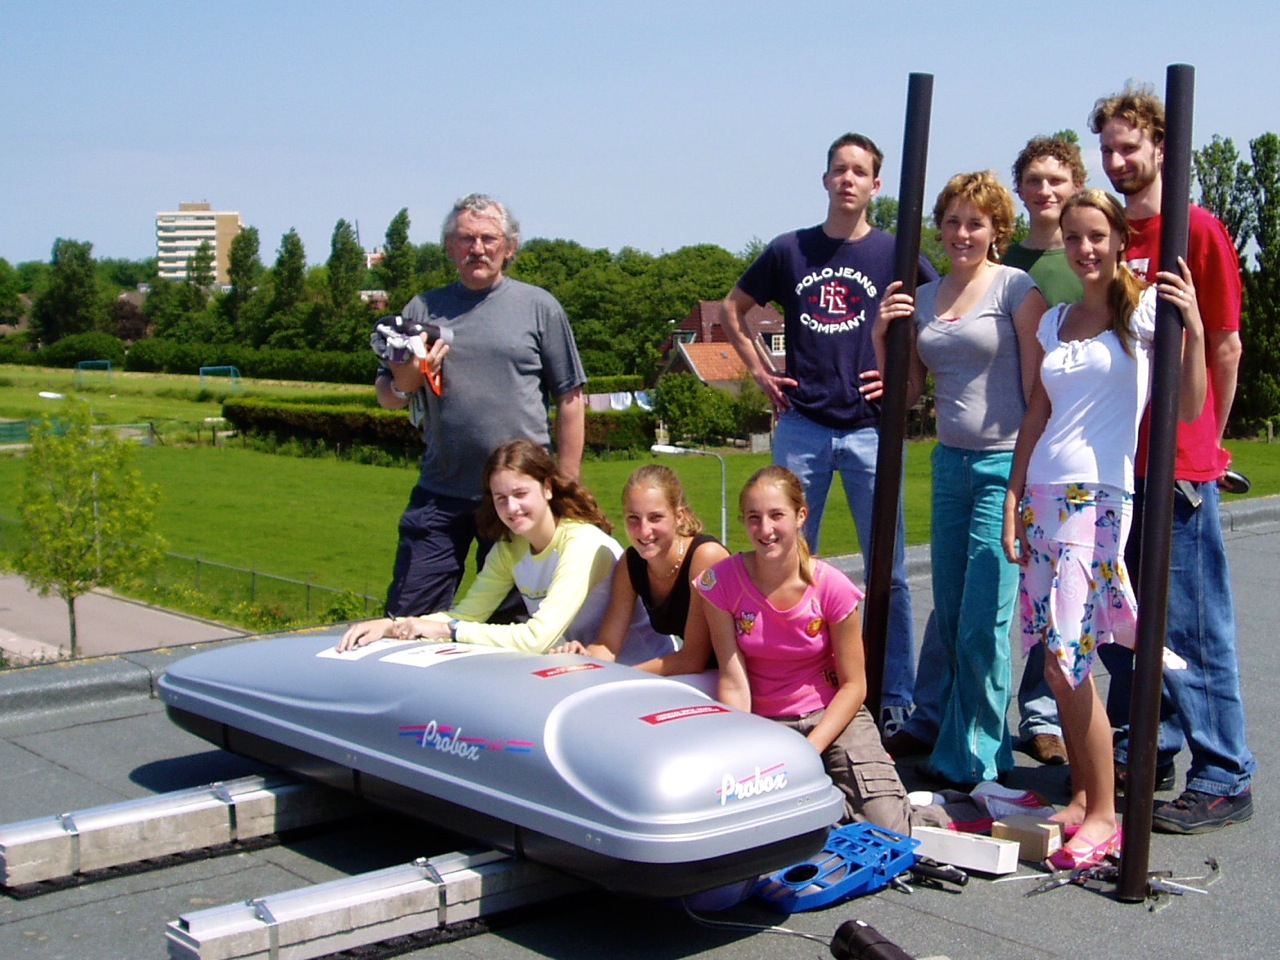
\includegraphics[width=\linewidth]{figures/students.jpg}
\caption{High-school students and their teacher with one of the \hisparc
detectors, at the Bonhoeffer College, in Castricum.  Photo courtesy of B. van
Eijk.}
\label{fig:students}
\end{figure}

Once a year, the \hisparc project organizes a national symposium. Students
present their research and the group giving the best presentation receives an award.
Furthermore, students take part in hands-on analysis sessions.

Students participating in \hisparc obtain a clearer picture of what
actual scientific research involves and are more interested in pursuing a
scientific career.  The decision to take part in \hisparc is, in the majority
of cases, made by the teachers, not their students.  This rules out the
possibility that the students were more inclined towards research beforehand and
joined the \hisparc project because of that.

\hisparc currently consists of close to a hundred stations concentrated around
scientific institutes in major cities in the Netherlands. The project has
stations in Denmark, the UK and even Vietnam. \hisparc also deploys weather
stations and lightning detectors. Unique to \hisparc, cosmic ray and particle
physics have been integrated in the curriculum of participating schools. There
are NiNa\footnote{Nieuwe Natuurkunde} modules for cosmic ray physics
\cite{NiNa-module},
as well as a series of topical letters for students and teachers
(RouteNet) \cite{RouteNet}. Recently, revised teaching materials have been
certified as an approved module for the NLT (Nature, Life and
Science)\footnote{Natuur, Leven en Technologie} secondary education subject. All
schools in the Netherlands can now teach cosmic ray physics as part of their
examination program \cite{NLT-module}.

The Dutch Foundation for Fundamental Research on Matter (FOM) has funded a
program to enable teachers to conduct research at a scientific institute or
university.
Teachers perform research during one year for one day a week, in close
collaboration with scientific staff. The \hisparc project has been a popular
choice for teachers and has worked with 6 to 7 teachers each year for the past
four years \cites{LIO:2009}{LIO:2010}{LIO:2011}. Research projects include
analyzing \hisparc data to determine the effect of atmospheric variables and the
evolution of the detector response over time. Teachers have also studied the
feasibility of applying pixel detectors (MPPCs) as alternatives to PMTs.

The scientific premise underlying sparse but large detector arrays is the detection of
large-scale correlated effects, like the Gerasimova-Zatsepin effect, short
bursts of showers, or other, as yet unknown, phenomena.  Deploying cosmic ray
detectors at high schools naturally creates a large and sparse array with
detectors situated at locations with interested and knowledgeable people willing to
maintain them. As a spin-off, electronics developed for \hisparc are now applied
in the Auger Radio experiment \cite{Coppens:2009} and EPR spectroscopy
\cite{FLARE}.
